\documentclass[journal]{IEEEtran}
\usepackage[T1]{fontenc}
\usepackage[utf8]{inputenc}
\usepackage{cite}
\usepackage{amsmath,amssymb}
\usepackage{graphicx}
\usepackage{booktabs}
\usepackage{array}
\usepackage{tabularx}
\usepackage{url}
\usepackage{xcolor}

\setlength{\textfloatsep}{7pt plus 1pt minus 2pt}
\setlength{\floatsep}{7pt plus 1pt minus 2pt}
\setlength{\intextsep}{7pt plus 1pt minus 2pt}
\setlength{\abovecaptionskip}{3pt}
\setlength{\belowcaptionskip}{0pt}
\setlength{\abovedisplayskip}{5pt plus 1pt minus 2pt}
\setlength{\belowdisplayskip}{5pt plus 1pt minus 2pt}
\renewcommand{\textfraction}{0.08}
\renewcommand{\topfraction}{0.92}
\renewcommand{\dbltopfraction}{0.92}
\renewcommand{\floatpagefraction}{0.8}
\renewcommand{\dblfloatpagefraction}{0.8}
\newcolumntype{Y}{>{\raggedright\arraybackslash}X}
\newcolumntype{L}[1]{>{\raggedright\arraybackslash}p{#1}}
\raggedbottom

\title{Rendezvous-Aware Route Choice for Urban Ride-Pooling Under Occlusion}
\author{Anonymous Authors}

\begin{document}
\maketitle
\vspace{-0.8em}

\begin{abstract}
Route choice in ride-pooling is often valued through corridor exposure alone: a route is considered attractive if it passes near more potentially compatible riders. This paper argues that such a view is incomplete in dense urban settings, where riders who appear near a route may still lack a practical, reliable common pickup opportunity. We therefore study route choice through route-induced rendezvous opportunity sets rather than through near-route riders alone. The study combines New York City taxi demand, Open Source Routing Machine alternatives, a hexagonal hierarchical spatial grid, route-anchor meeting opportunities, and an urban-context proxy built from official street centerline, sidewalk, building-footprint, land-use, and elevation layers. Feasible meeting opportunities are filtered by walk accessibility, timing, and remaining trip value, while observable opportunities are discounted by a calibrated pickup-success model under occlusion. Evaluation includes a controlled single-driver study, a secondary rolling-dispatch validation, matched within-driver route-pair analysis, Green-domain transfer, and curated local-geometry case studies. Corridor-only valuation is consistently weakest and exhibits a much larger nominal-versus-realized gap than the rendezvous-aware policies. The main gain comes from replacing corridor exposure with feasible rendezvous opportunities, while observability-aware valuation is most useful in sparse, high-occlusion regimes and in a harder morning-peak slice. The central conclusion is therefore not that observability dominates universally, but that route choice should be evaluated through feasible and observable rendezvous opportunities rather than through proximity alone.
\end{abstract}

\begin{IEEEkeywords}
ride-pooling, rendezvous, route choice, urban occlusion, meeting-point selection, H3
\end{IEEEkeywords}

\section{Introduction}
\IEEEPARstart{R}{oute}-aware ride-pooling is usually framed as a question of exposure: if a driver takes route A rather than route B, which riders lie near the resulting corridor \cite{santi2014,alonso2017}? That view is operationally useful, but incomplete. In dense urban settings, riders who appear near a route are not automatically serviceable. Some cannot reach a good common pickup location under the timing budget; others can reach such a point, but only at meeting opportunities that are difficult to observe, difficult to coordinate, or unreliable under urban morphology.

This paper studies route choice through that missing layer. The key object is not the near-route rider and not the meeting point in isolation, but the \emph{route-induced set of feasible and observable rendezvous opportunities}. A route is valuable because it exposes a structured set of common meeting opportunities. Those opportunities can be more or less accessible and more or less observable. Once that structure is made explicit, route choice becomes a decision problem over route-induced opportunity sets rather than a problem of corridor membership alone.

This framing places the paper between several neighboring literatures. Dynamic ride-pooling has focused heavily on assignment, pooling feasibility, and rolling dispatch \cite{agatz2012,alonso2017}. Meeting-point work has shown that pickup flexibility matters materially \cite{stiglic2016,stumpe2024,zhou2026}. Route recommendation work has shown that the geometry of a route can change matching outcomes \cite{bassem2022,xia2019}. The present paper combines those ideas into one narrower question: given multiple feasible routes for a driver, which route creates the best realized ride-pooling outcome once corridor exposure, rendezvous feasibility, and observability under occlusion are all taken into account?

The contribution is intentionally a systems and decision-making contribution, not a full perception contribution. We do not claim to solve urban sensing or pickup coordination in all of its physical detail. Instead, we ask whether a structured observability layer changes route value in a meaningful way, and whether that change survives stronger baselines and harder operating regimes.

The paper makes four contributions:
\begin{enumerate}
\item It reframes route choice around \emph{route-induced rendezvous opportunity sets}, distinguishing corridor exposure, rendezvous feasibility, and observability under occlusion.
\item It presents a reproducible implementation that combines OSRM route alternatives \cite{osrmapi}, H3 corridor and anchor geometry \cite{h3docs}, NYC Yellow demand \cite{azureyellow}, and an H3-aggregated urban-context layer for occlusion-aware evaluation.
\item It evaluates the formulation against stronger deterministic baselines and a secondary ML comparator in both a controlled single-driver setting and a repaired rolling-dispatch setting with failed-attempt retirement.
\item It shows that corridor-only valuation overstates service value, that rendezvous feasibility is the main performance jump, and that observability-aware valuation is most useful in sparse, high-occlusion regimes rather than uniformly in all regimes.
\end{enumerate}

Section II reviews related work. Section III formalizes route-induced rendezvous opportunities. Section IV describes the implementation and policy family. Section V details the experimental design. Section VI reports the empirical results. Section VII discusses interpretation and positioning. Section VIII states limitations, and Section IX concludes.
\section{Related Work}
Dynamic ride-sharing and ride-pooling have been studied primarily through assignment, feasibility, and dispatch. Agatz \emph{et al.} surveyed dynamic ride-sharing optimization and emphasized the interaction between temporal compatibility and operating constraints \cite{agatz2012}; their earlier simulation work also showed that stronger decision rules can materially outperform naive baselines \cite{agatz2011}. Alonso-Mora \emph{et al.} demonstrated the value of online trip--vehicle assignment at high capacity \cite{alonso2017}. Santi \emph{et al.} and Tachet \emph{et al.} showed that shareability is highly sensitive to temporal windows and density \cite{santi2014,tachet2017}. Those results motivate our realism-first distinction between nominal corridor exposure and realized serviceability.

Meeting-point flexibility is especially relevant to our setting. Stiglic \emph{et al.} showed that dynamic ride-sharing performance depends strongly on driver and rider flexibility \cite{stiglic2016}. More recent work on shared pickup and drop-off design has further shown that meeting-point choice changes both operational efficiency and usability \cite{stumpe2024,zhou2026}. Our paper does not optimize arbitrary pickup designs or solve a full pickup-location problem. Instead, it asks how a \emph{route} should be valued once the meeting opportunities it induces are taken seriously.

Route recommendation and route-aware matching form the third neighboring strand. Bassem \emph{et al.} studied route recommendation as a lever for carpool facilitation \cite{bassem2022}, and Xia \emph{et al.} showed that route structure interacts with social and route networks in carpool matching \cite{xia2019}. In ride-service operations, route and dispatch decisions have also been explored through systematic optimization and search-based methods \cite{chen2021}. The difference in the present work is the primitive: we do not treat route quality as rider exposure alone, but as a function of the feasible and observable rendezvous opportunities created by each route.

\section{Problem Setup}
\subsection{Entities and Route Alternatives}
Let $d \in \mathcal{D}$ denote a driver trip with departure time $t_d$, origin $o_d$, destination $q_d$, and seat capacity $Q_d$. Let $\mathcal{R}_d = \{r_{d1}, \ldots, r_{dK}\}$ denote the feasible OSRM route alternatives for driver $d$, with $K=3$ in the present evaluation. Each route $r \in \mathcal{R}_d$ is converted into:
\begin{enumerate}
\item an H3 corridor $C_r$, used for coarse nearby-rider exposure, and
\item an ordered set of route anchor cells $A_r = (a_1, \ldots, a_m)$, used to represent possible rendezvous opportunities.
\end{enumerate}

Let $u \in \mathcal{U}$ denote a rider request with pickup cell $h_u^p$, pickup time $t_u$, fare proxy $f_u$, passenger count $p_u$, and drop-off information used to estimate downstream remaining-trip value.

\begin{table}[t]
\caption{Notation used in the rendezvous-aware formulation.}
\label{tab:notation}
\centering
\footnotesize
\begin{tabularx}{\columnwidth}{L{0.27\columnwidth}Y}
\toprule
Symbol & Meaning \\
\midrule
$d \in \mathcal{D}$ & driver trip \\
$u \in \mathcal{U}$ & rider request \\
$\mathcal{R}_d$ & feasible route set for driver $d$ \\
$C_r$ & H3 corridor for route $r$ \\
$A_r$ & ordered route-anchor cells for route $r$ \\
$\Omega_r(u)$ & feasible rendezvous anchors for rider $u$ on route $r$ \\
$o_r(u,a)$ & observability score for rider $u$, route $r$, anchor $a$ \\
$p_r^{\mathrm{succ}}(u,a)$ & pickup success probability under occlusion \\
$\tilde v_r(u)$ & best rider-level opportunity value on route $r$ \\
$s_\phi(d,r)$ & route score under policy $\phi$ \\
$g(d,r)$ & realized scenario profit of launching driver $d$ on route $r$ \\
\bottomrule
\end{tabularx}
\end{table}

\subsection{From Corridor Exposure to Rendezvous Opportunity Sets}
The weakest route-aware notion is corridor exposure. A rider is corridor-near if the rider's pickup cell lies in the expanded route corridor:
\[
\mathcal{U}_r^{\mathrm{corr}} = \{u \in \mathcal{U} \mid h_u^p \in C_r,\; |t_u - t_d| \le \tau_{\mathrm{req}}\}.
\]
This is enough to recover the classical route-aware view: a route is attractive if it passes near more riders.

The paper's main move is to replace corridor-near riders with route-induced rendezvous opportunities. For rider $u$ and route $r$, define the feasible opportunity set
\[
\Omega_r(u) = \left\{ a \in A_r \;\middle|\; \mathrm{dist}_{\mathrm{H3}}(h_u^p,a) \le \kappa_m,\; w(u,a) \le \tau_{\mathrm{walk}},\; \rho_r(u,a) \ge \tau_{\mathrm{remain}} \right\},
\]
where $\kappa_m$ is the meeting neighborhood, $w(u,a)$ is rider walk time to anchor $a$, and $\rho_r(u,a)$ is the remaining downstream trip value after intercepting route $r$ at anchor $a$. A rider is rendezvous-feasible for route $r$ only if $\Omega_r(u)$ is non-empty.

This shift matters because a route can expose many corridor-near riders while exposing relatively few workable common meeting opportunities. The corridor-only view therefore tends to overestimate apparent matchability.

\subsection{Observability Under Occlusion}
Feasible opportunities are not equally reliable. For each feasible anchor $a \in \Omega_r(u)$, the system computes an observability score
\[
o_r(u,a) \in [0,1],
\]
from route-local geometry and urban context. The implementation combines local straightness, turn severity, anchor ambiguity, anchor clutter, sidewalk access, and building-height / urban-clutter proxies. The calibrated core weight profile used in the experiments is 0.20 for straightness, 0.30 for turn severity, 0.30 for ambiguity, and 0.20 for clutter; the auxiliary context features modulate those components.

Observability is converted into a pickup-success probability through a clipped occlusion model:
\[
p_r^{\mathrm{succ}}(u,a) = \operatorname{clip}\left(0.95 - \lambda_{\mathrm{occ}}(1-o_r(u,a)),\; 0.35,\; 0.95\right),
\]
where $\lambda_{\mathrm{occ}}$ controls scenario severity. The paper does not claim this is a full sensing model. It is a structured route-level uncertainty model that makes observability decision-relevant.

\subsection{Route Valuation Views}
Given a feasible route $r$, the rider-level best opportunity value is
\[
\tilde v_r(u) = \max_{a \in \Omega_r(u)} v_r(u,a),
\]
where $v_r(u,a)$ depends on the policy family.

The three conceptual route-valuation views are:
\begin{enumerate}
\item \textbf{Corridor-only valuation.} Route score depends on corridor-near rider exposure only.
\item \textbf{Rendezvous-aware valuation.} Route score depends on feasible opportunities with no observability discount.
\item \textbf{Rendezvous + observability valuation.} Route score depends on feasible opportunities discounted by pickup reliability under occlusion.
\end{enumerate}

The evaluation also includes stronger deterministic baselines and a secondary ML comparator, but these three views remain the scientific backbone of the paper.

\subsection{Route-Value Objective and Two Propositions}
The route-choice decision solved by policy family $\phi$ is
\[
r_d^\star(\phi) = \arg\max_{r \in \mathcal{R}_d} s_\phi(d,r), \qquad
s_\phi(d,r) = \sum_{u \in \mathcal{U}_r^{\mathrm{corr}}} \tilde v_r^\phi(u) - c(r),
\]
where $c(r)$ is route operating cost and $\tilde v_r^\phi(u)$ depends on whether policy $\phi$ values exposure only, feasibility only, or feasibility plus observability. Realized value is then obtained by sampling pickup outcomes from the selected route-specific opportunity set.

\textbf{Proposition 1.} \emph{If a nontrivial share of corridor-near riders have empty feasible rendezvous sets, then corridor-only valuation overstates realized route value relative to rendezvous-aware valuation.}

\emph{Intuition.} Corridor-only scoring counts riders before the common meeting problem is solved. When many corridor-near riders cannot actually intercept the route through any admissible anchor, the corridor-only score includes opportunity mass that cannot convert into realized service. This is exactly the nominal-versus-realized gap measured in the experiments.

\textbf{Proposition 2.} \emph{Observability-aware and observability-blind valuation coincide as $\lambda_{\mathrm{occ}}\rightarrow 0$, and diverge as cross-anchor observability heterogeneity increases.}

\emph{Intuition.} When occlusion is negligible, the pickup-success discount approaches a constant and observability ceases to reorder anchors or routes. As route-induced opportunity sets become more heterogeneous in observability, the discount becomes selective and route ordering can change even when corridor exposure and feasible opportunity counts remain similar.
\section{Implementation and Policy Family}
\subsection{Route Corridors, Anchors, and Candidate Retrieval}
Each driver route is requested through OSRM \cite{osrmapi}, densified into an ordered polyline, and mapped to H3 resolution 9 cells \cite{h3docs}. The corridor is built with a one-ring expansion ($\kappa_c=1$), while meeting opportunities use anchor cells on the ordered route spine plus a one-ring meeting neighborhood ($\kappa_m=1$). Candidate riders are first retrieved by pickup proximity to the corridor and exact request-time compatibility. Unlike the earlier corridor paper, the present pipeline does not require both pickup and drop-off to lie in the corridor; pickup retrieval is corridor-centric, and downstream trip value is handled later as part of rendezvous feasibility.

For each corridor-near rider, the implementation evaluates route anchors as potential common meeting opportunities. An anchor is feasible only if it satisfies the meeting neighborhood, walk-time, and remaining-trip conditions. This produces a route-specific opportunity set rather than a rider-only candidate set.

\subsection{Observability Proxy and Calibration}
The observability proxy combines two sources of information. The first is route-local geometry: straightness, turn severity, ambiguity among anchors, and clutter around the anchor. The second is urban context aggregated to H3 from official NYC street centerline, sidewalk centerline, building footprint, PLUTO, and elevation layers. The resulting context table supports clutter, sidewalk-access, and morphology proxies without requiring explicit sensor simulation.

To reduce arbitrariness, the study calibrates the core observability weights on non-test meeting-point data. A larger Yellow meeting-point dataset with 19,798 rows is split into train, validation, and test partitions. The calibration routine performs a coarse simplex search over the core weights and selects the profile that best improves predictive quality on non-test data. The chosen profile slightly improves test Brier score from 0.13636 to 0.13634 and test ROC AUC from 0.5348 to 0.5403. Although the lift is small, it makes the observability layer less heuristic and more defensible.

\subsection{Policies}
Table~\ref{tab:policies} summarizes the policy family evaluated in the study.

\begin{table}[t]
\caption{Route-selection policies used in the paper.}
\label{tab:policies}
\centering
\footnotesize
\begin{tabularx}{\columnwidth}{L{0.28\columnwidth}Y}
\toprule
Policy & Route-scoring intuition \\
\midrule
\texttt{corridor\_only} & prefer routes exposing more corridor-near riders; serves as the weakest route-aware baseline \\
\texttt{time\_only\_baseline} & prefer shorter or faster routes without explicit rendezvous valuation \\
\texttt{feasible\_count\_baseline} & prefer routes exposing more feasible rendezvous opportunities \\
\texttt{walk\_aware\_rendezvous} & prefer feasible opportunities with stronger walk convenience \\
\texttt{rendezvous\_only} & value the best feasible opportunity per rider without observability discount \\
\texttt{rendezvous\_observable} & value feasible opportunities discounted by pickup success under occlusion \\
\texttt{ml\_meeting\_point\_comparator} & secondary comparator that learns a meeting-point ranking proxy from geometry and context features \\
\bottomrule
\end{tabularx}
\end{table}

Two implementation details matter for credibility. First, the repaired pipeline keeps a true corridor-only realized baseline: corridor-near riders can still fail later because no workable rendezvous anchor exists. Second, seat assignment is no longer greedy in a potentially misleading way; the system uses optimal small-capacity packing over rider-level opportunity values.

\subsection{Rolling Dispatch Layer}
The primary evidence layer is the controlled single-driver study, but the paper also uses a rolling-dispatch validation because route choice interacts with competition for a shared rider pool. Dispatch proceeds in fixed batches. Within each batch, riders are exclusive and failed attempts are retired rather than left open for repeated retries. This repaired exclusivity model makes the dispatch evidence materially more trustworthy than the earlier draft stack.

\section{Experimental Design}
\subsection{Demand, Urban Context, and Scenarios}
The primary demand source is NYC TLC Yellow data \cite{azureyellow}. Long trips serve as proxy drivers and shorter trips serve as proxy riders, following the same public-data logic as the earlier route-aware work, but the present paper is centered on route-induced meeting opportunities rather than corridor exposure. The urban-context layer is aggregated to H3 so that demand, routes, and observability features share a common spatial frame.

The headline all-day scenarios are:
\begin{enumerate}
\item \textbf{Primary}: rider density 100, occlusion $\lambda=0.25$,
\item \textbf{Sparse high occlusion}: rider density 10, occlusion $\lambda=0.40$,
\item \textbf{Very sparse low occlusion}: rider density 10, occlusion $\lambda=0.10$,
\item \textbf{Very sparse extreme occlusion}: rider density 10, occlusion $\lambda=0.55$.
\end{enumerate}

The robustness pass re-runs sparse high occlusion in morning peak (07:00--10:00) and evening peak (16:00--19:00) slices, and it adds a second-domain transfer check on NYC Green. The Green pass reuses the Yellow-calibrated observability profile rather than recalibrating on the robustness domain, so the transfer exercise tests portability rather than additional tuning.

\begin{table}[t]
\caption{Primary scenario assumptions used in the study.}
\label{tab:assumptions}
\centering
\footnotesize
\begin{tabularx}{\columnwidth}{L{0.32\columnwidth}L{0.22\columnwidth}Y}
\toprule
Component & Default & Notes \\
\midrule
Demand domain & NYC Yellow & April test split for evaluation \\
Route alternatives & 3 & genuine OSRM alternatives when available \\
H3 resolution & 9 & shared by routes, riders, and urban context \\
Corridor neighborhood & $\kappa_c=1$ & one-ring corridor exposure \\
Meeting neighborhood & $\kappa_m=1$ & one-ring anchor access \\
Maximum walk time & 6 min & feasibility filter for rendezvous anchors \\
Single-driver evaluation & 500 drivers $\times$ 5 seeds & all all-day scenarios at full route coverage \\
Dispatch evaluation & 500 drivers $\times$ 5 seeds for primary; 250 drivers $\times$ 3 seeds otherwise & secondary systems validation \\
Robustness slices & morning / evening peak & sparse high occlusion only \\
Green robustness & 500 drivers $\times$ 5 seeds single-driver, 250 drivers $\times$ 3 seeds dispatch & Yellow-calibrated observability profile transferred unchanged \\
\bottomrule
\end{tabularx}
\end{table}

\subsection{Evaluation Layers}
The paper uses two complementary evidence layers.
\begin{enumerate}
\item \textbf{Controlled single-driver study.} This is the primary evidence layer. Each policy sees the same driver, route set, rider snapshot, and seed, isolating the effect of route valuation itself.
\item \textbf{Rolling dispatch validation.} This is the secondary systems layer. It checks whether the route-ordering signal survives rider exclusivity and overlapping competition among drivers.
\end{enumerate}

This split is important. The single-driver study answers whether route-induced rendezvous valuation changes route quality. The dispatch layer answers whether that change remains meaningful once drivers compete for the same request pool.

\subsection{Metrics and Statistical Reporting}
The main single-driver metric is mean actual profit. The dispatch layer reports mean profit per driver, service rate, wait time, and walk time. For the route-choice study, the paper also reports the mean nominal-versus-realized gap:
\[
\Delta_{\mathrm{gap}} = \mathbb{E}[\text{nominal route value} - \text{realized route value}],
\]
which is central to the corridor-only critique.

Bootstrap 95\% intervals and paired policy deltas are computed from the per-driver results. The emphasis is on comparative evidence rather than on claiming calibrated financial forecasts.

\subsection{Matched-Pair and Case-Study Evaluation}
To isolate the observability claim from simple exposure differences, the paper adds a matched within-driver route-pair analysis in sparse high occlusion. Two route alternatives for the same driver are considered matched when their corridor exposure, feasible opportunity count, route distance, and mean walk burden remain close:
\[
|\Delta \text{candidate count}| \le 2, \quad
|\Delta \text{feasible count}| \le 1, \quad
\frac{|\Delta \text{distance}|}{\min(\text{distance})} \le 0.10, \quad
|\Delta \text{walk}| \le 0.5 \text{ min}.
\]
Within each matched pair, the higher-observability route is compared against the lower-observability route under repeated realized pickup draws using the same saved opportunity sets. This provides a cleaner mechanism check than aggregate policy bars alone.

The paper also adds a curated local-geometry validation layer. Eight matched route pairs are selected for case-study panels, with preference for Yellow morning-peak sparse high occlusion and then Green all-day sparse high occlusion when available. Each panel uses only local reproducible overlays: route geometry, corridor cells, candidate anchors, selected anchors, building footprints, and sidewalk centerlines. A fixed rubric scores approach legibility, anchor ambiguity, sidewalk continuity, and local openness on a 1--3 scale.
\section{Results}
\subsection{Single-Driver Headline Results}
Figure~\ref{fig:primary} and Figure~\ref{fig:strongbaselines} summarize the main route-choice evidence. In the primary calibrated all-day regime, \texttt{corridor\_only} achieves mean actual profit 6.76, while the stronger deterministic baselines range from 16.03 to 17.30 and the rendezvous-aware policies reach 17.60 (\texttt{rendezvous\_only}) and 17.57 (\texttt{rendezvous\_observable}). The first important result is therefore not about observability; it is that corridor-only valuation dramatically underperforms once the route is judged by realized service value rather than by nominal exposure.

Figure~\ref{fig:gap} makes that point especially clear. In the primary regime, the corridor-only baseline shows a nominal-versus-realized gap of 18.46, while the rendezvous-aware methods stay near 3.55. This is exactly the gap the paper is about: a corridor-only route can appear rich in opportunity while exposing relatively few practical meeting opportunities.

The paper's headline regime is sparse high occlusion. In the all-day slice, the full ordering is -3.39 for \texttt{corridor\_only}, -1.64 for \texttt{time\_only\_baseline}, -1.01 for \texttt{feasible\_count\_baseline}, -0.79 for \texttt{walk\_aware\_rendezvous}, -0.70 for \texttt{rendezvous\_only}, and -0.68 for \texttt{rendezvous\_observable}. Even though the regime is hard enough that absolute profits fall below zero, the route-ordering result remains meaningful: relative to corridor-only valuation, observability-aware rendezvous valuation improves mean actual profit by 2.71 with bootstrap interval [2.43, 3.00]. Relative to \texttt{rendezvous\_only}, the mean gain is only 0.025 with an interval that still overlaps zero. The aggregate bar-chart story therefore remains modest but positive.

That is why the matched route-pair analysis matters. Figure~\ref{fig:mechanism} shows a representative within-driver route pair in which corridor exposure and feasible opportunity count are similar, but anchor quality and local geometry differ. Figure~\ref{fig:matched} then summarizes the full matched analysis. In all-day sparse high occlusion, the higher-observability route exceeds its matched lower-observability alternative by 5.28 mean realized-profit units with 95\% interval [4.21, 6.37]. In the morning-peak slice, the corresponding mean delta is 0.89 with interval [0.06, 1.71]. This is the cleanest direct evidence that observability changes route value even when simple exposure and feasibility counts are held approximately fixed.

\begin{figure}[t]
\centering
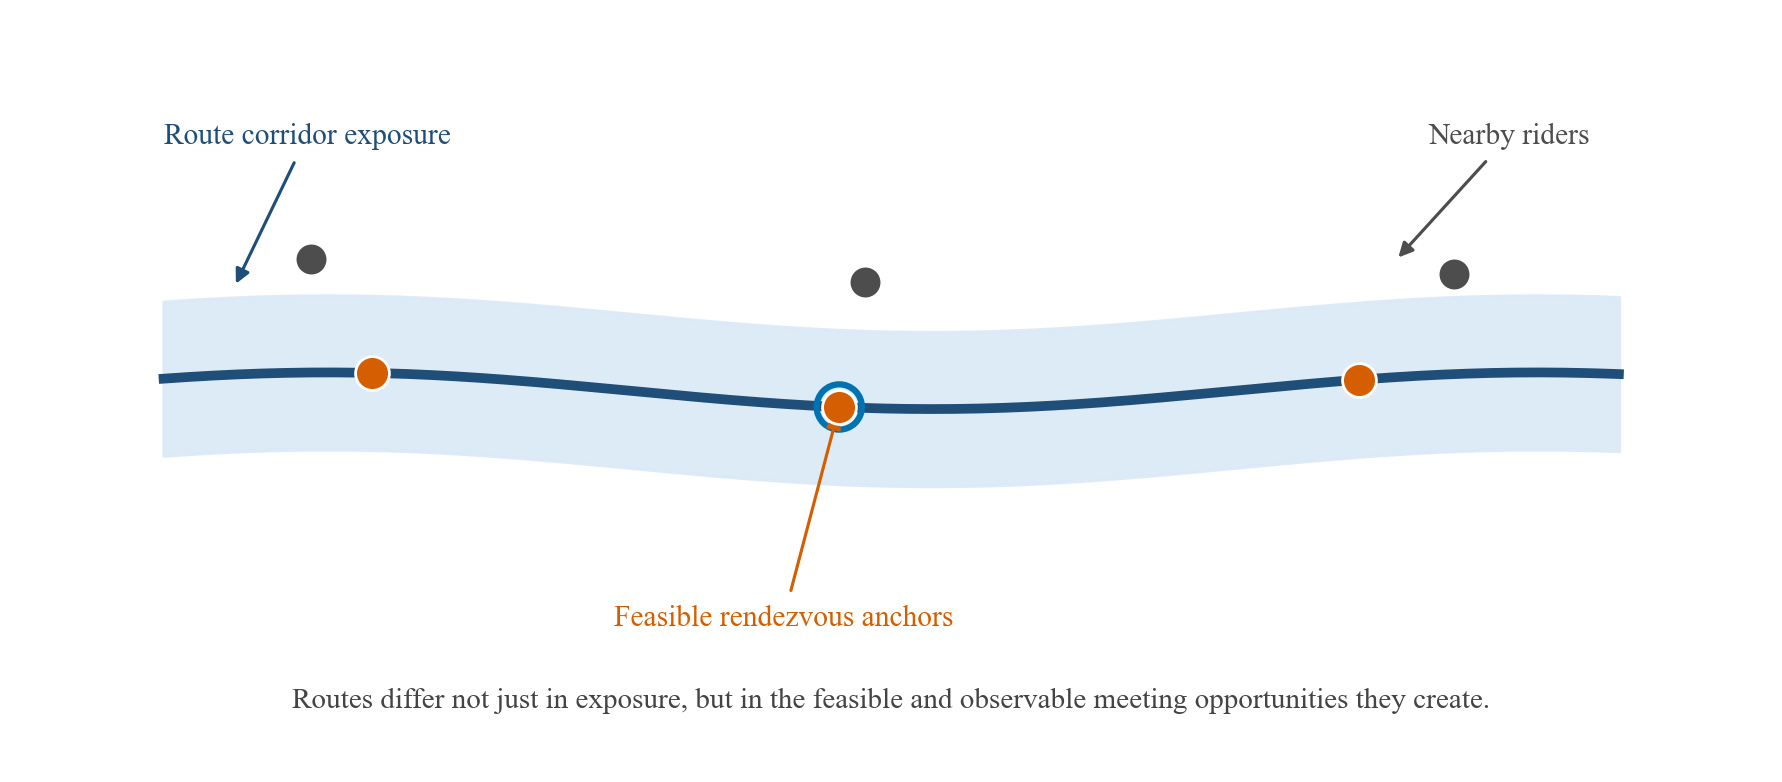
\includegraphics[width=\columnwidth]{figures/rendezvous_fig1_concept.png}
\caption{Conceptual view of route-induced rendezvous opportunities. Corridor exposure is the weakest layer; feasible and observable anchors are the decision-relevant layers.}
\label{fig:concept}
\end{figure}

\begin{figure}[t]
\centering
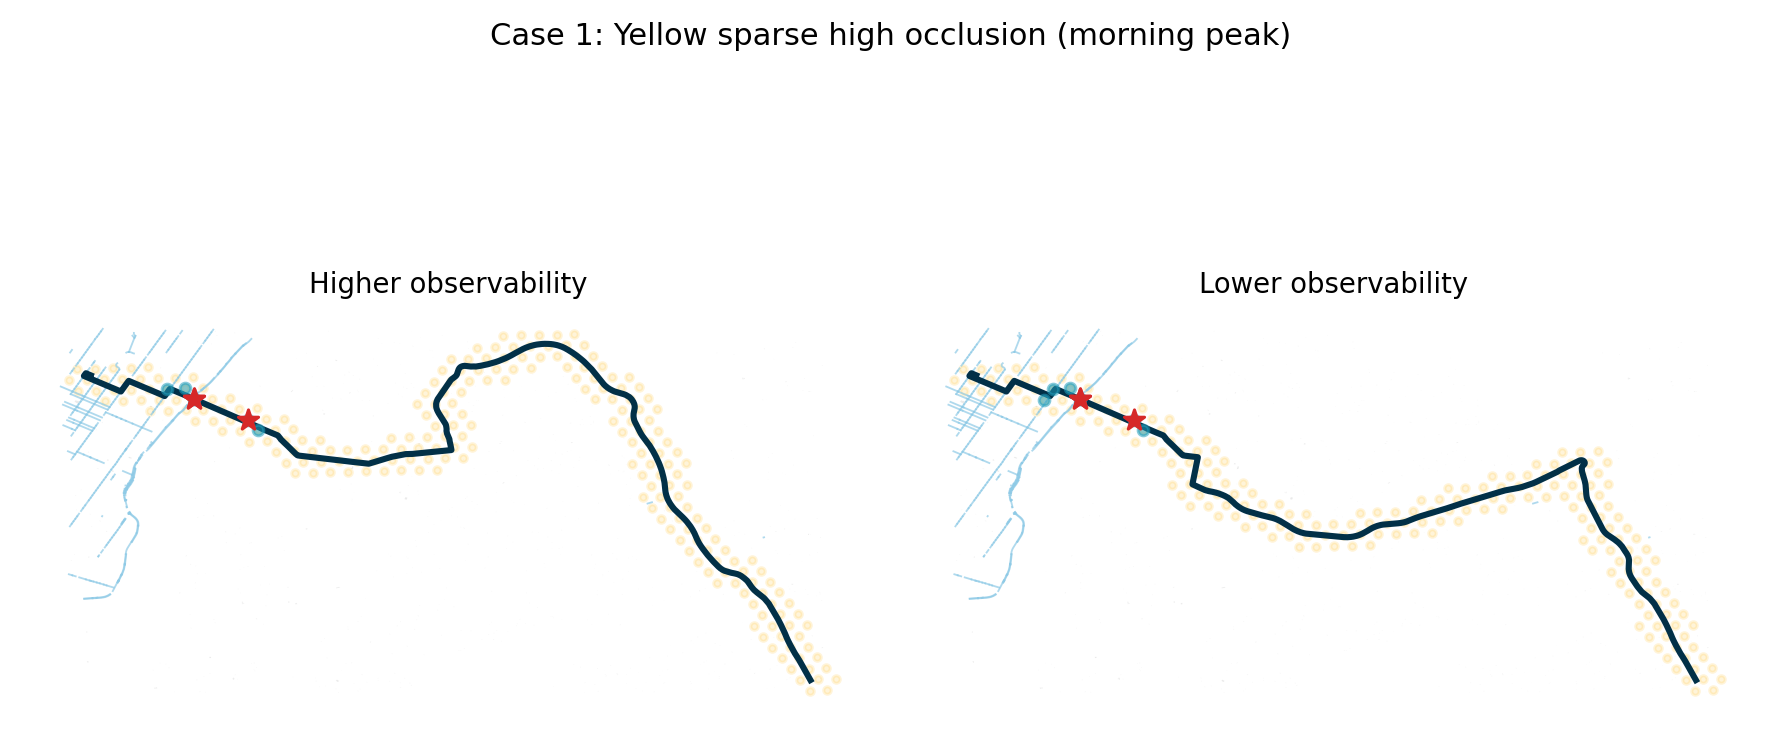
\includegraphics[width=\columnwidth]{figures/rendezvous_fig2_matched_pair_mechanism.png}
\caption{Representative matched route pair. The two routes expose similar opportunity volume, but the higher-observability route produces cleaner anchor geometry and better realized value.}
\label{fig:mechanism}
\end{figure}

\begin{figure}[t]
\centering
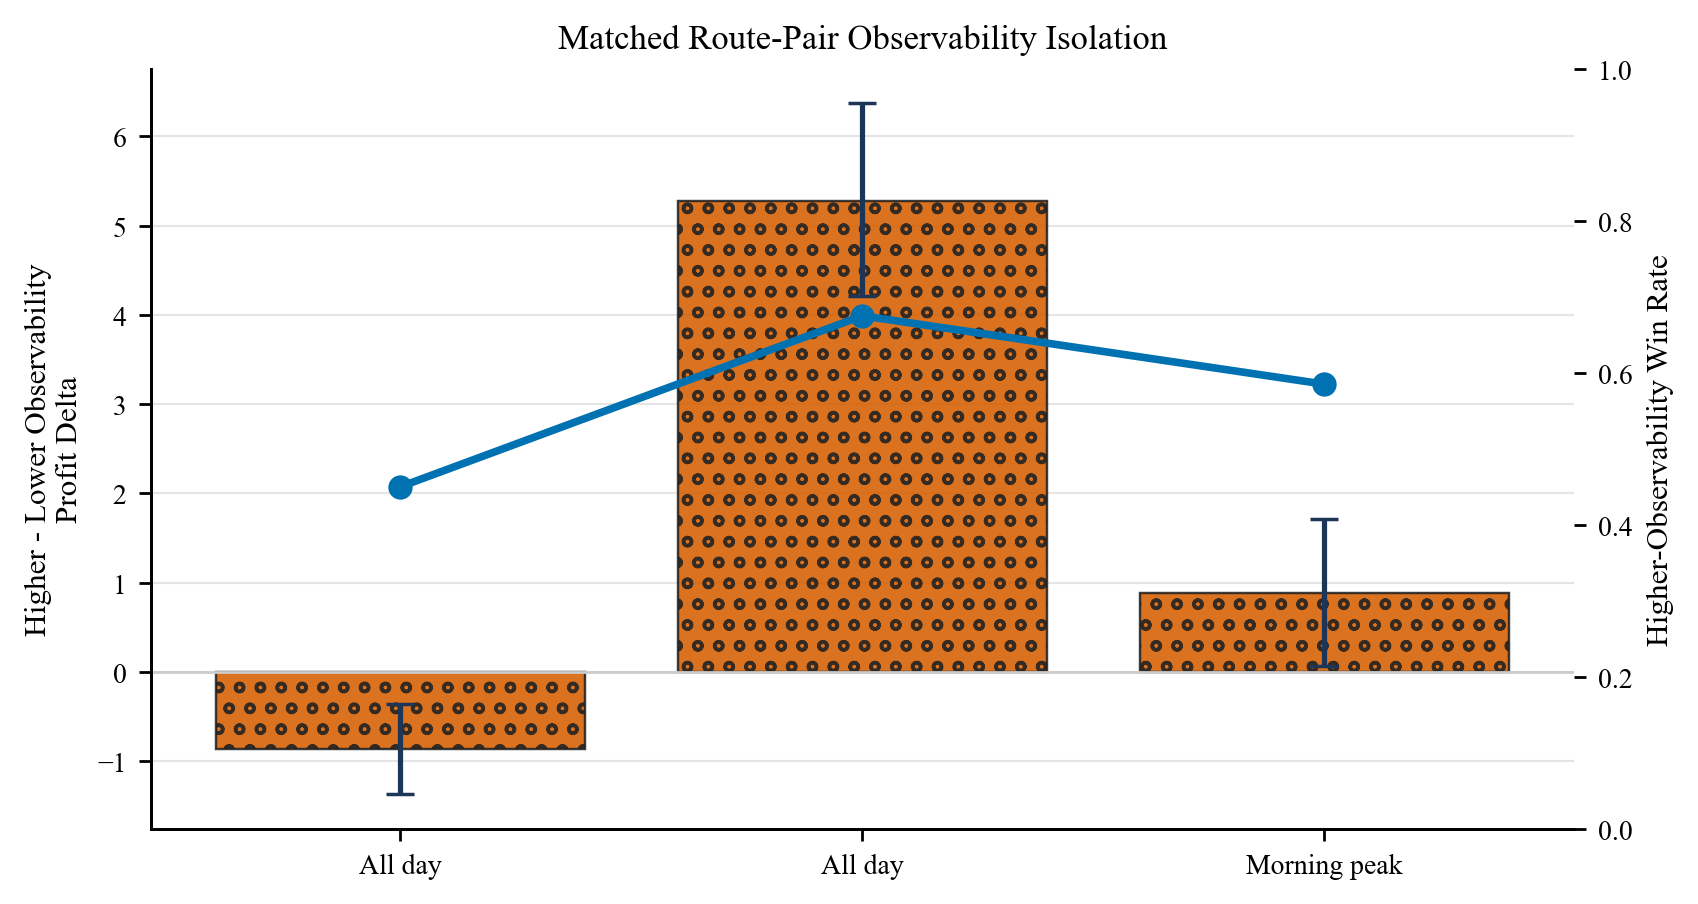
\includegraphics[width=\columnwidth]{figures/rendezvous_fig2_matched_pairs.png}
\caption{Matched within-driver observability analysis in sparse high occlusion. Higher-observability routes beat lower-observability alternatives in both all-day and morning-peak slices.}
\label{fig:matched}
\end{figure}

\begin{figure}[t]
\centering
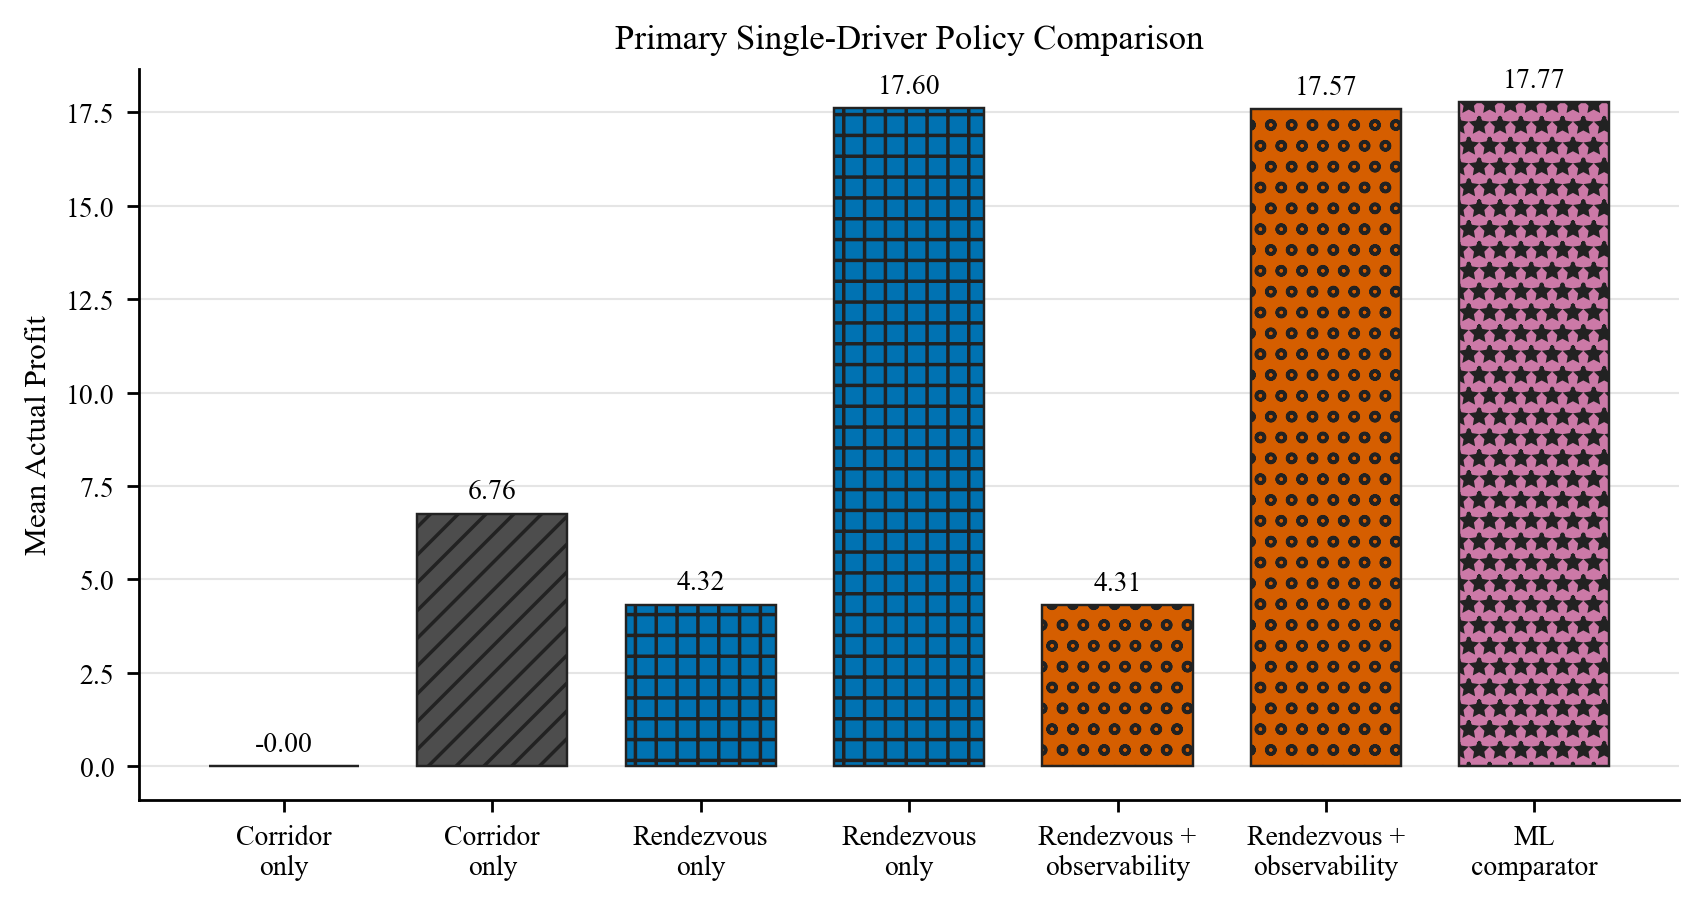
\includegraphics[width=\columnwidth]{figures/rendezvous_fig2_primary.png}
\caption{Primary single-driver comparison. The largest jump is from corridor-only valuation to rendezvous-aware valuation.}
\label{fig:primary}
\end{figure}

\begin{figure}[t]
\centering
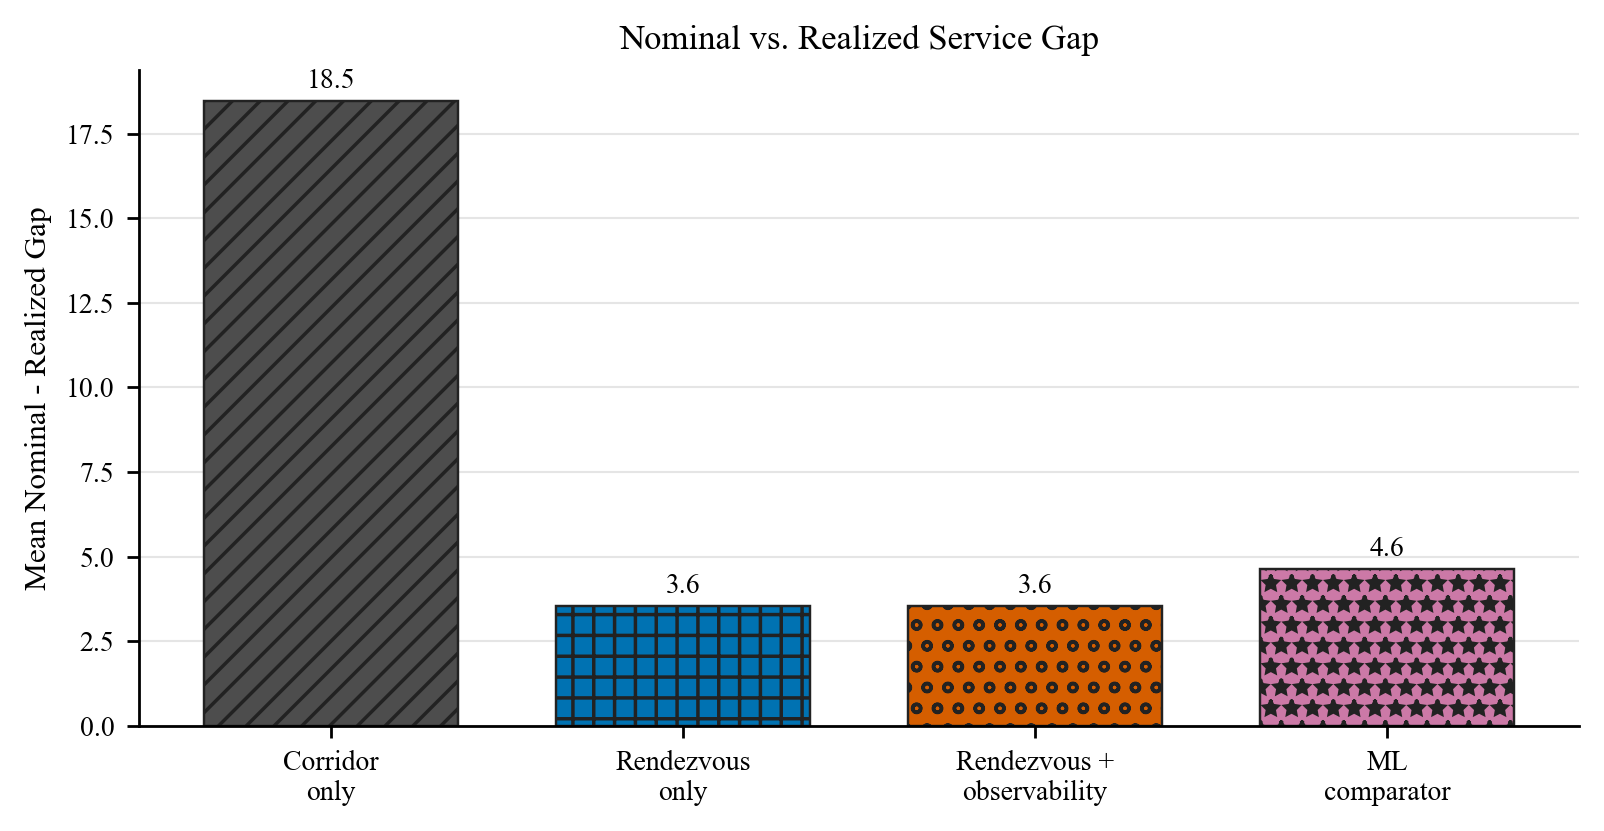
\includegraphics[width=\columnwidth]{figures/rendezvous_fig3_gap.png}
\caption{Nominal versus realized service gap in the primary regime. Corridor-only valuation materially overstates route value.}
\label{fig:gap}
\end{figure}

\begin{figure}[t]
\centering
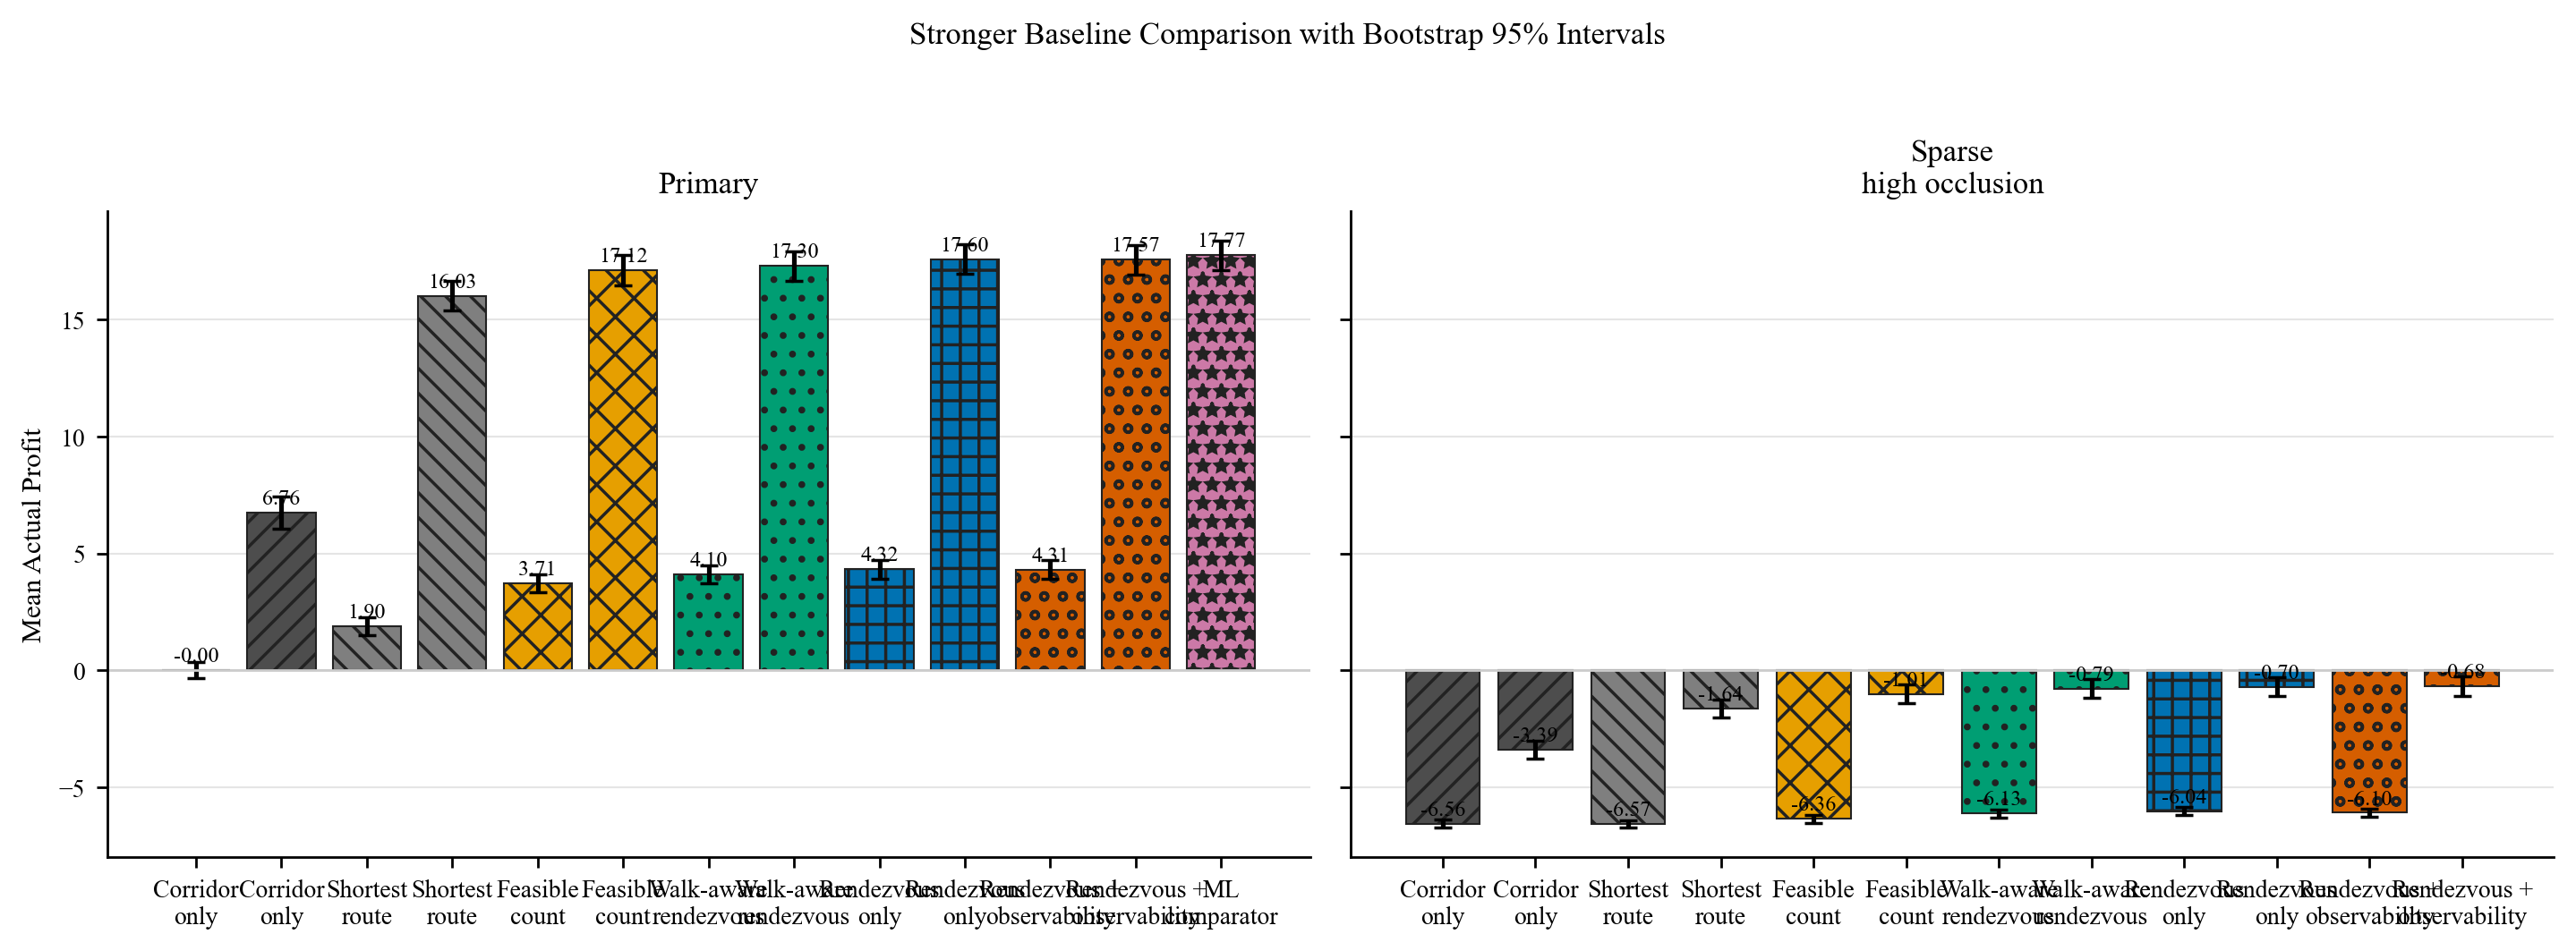
\includegraphics[width=\columnwidth]{figures/rendezvous_fig7_strong_baselines.png}
\caption{Stronger deterministic baseline comparison with bootstrap 95\% intervals. The hard-regime ordering survives after adding more credible competitor policies.}
\label{fig:strongbaselines}
\end{figure}

\subsection{Dispatch Validation}
Figure~\ref{fig:dispatch} shows that the same qualitative ordering survives in rolling dispatch. In primary dispatch, mean profit per driver is 3.87 for \texttt{corridor\_only}, 10.51 for \texttt{time\_only\_baseline}, 11.53 for \texttt{feasible\_count\_baseline}, 11.81 for \texttt{walk\_aware\_rendezvous}, 12.10 for \texttt{rendezvous\_only}, and 12.19 for \texttt{rendezvous\_observable}. In all-day sparse high occlusion, the corresponding values are -2.67, -0.97, 0.37, 0.41, 0.57, and 0.57.

The dispatch layer matters because it shows that the paper's core signal is not an artifact of isolated route scoring. Once failed attempts are retired and exclusivity is enforced, corridor-only valuation remains weakest, and the rendezvous-aware policies remain strongest. The dispatch gap between \texttt{rendezvous\_only} and \texttt{rendezvous\_observable} is again modest, but the direction still favors observability-aware valuation in the headline hard regime.

\begin{figure}[t]
\centering
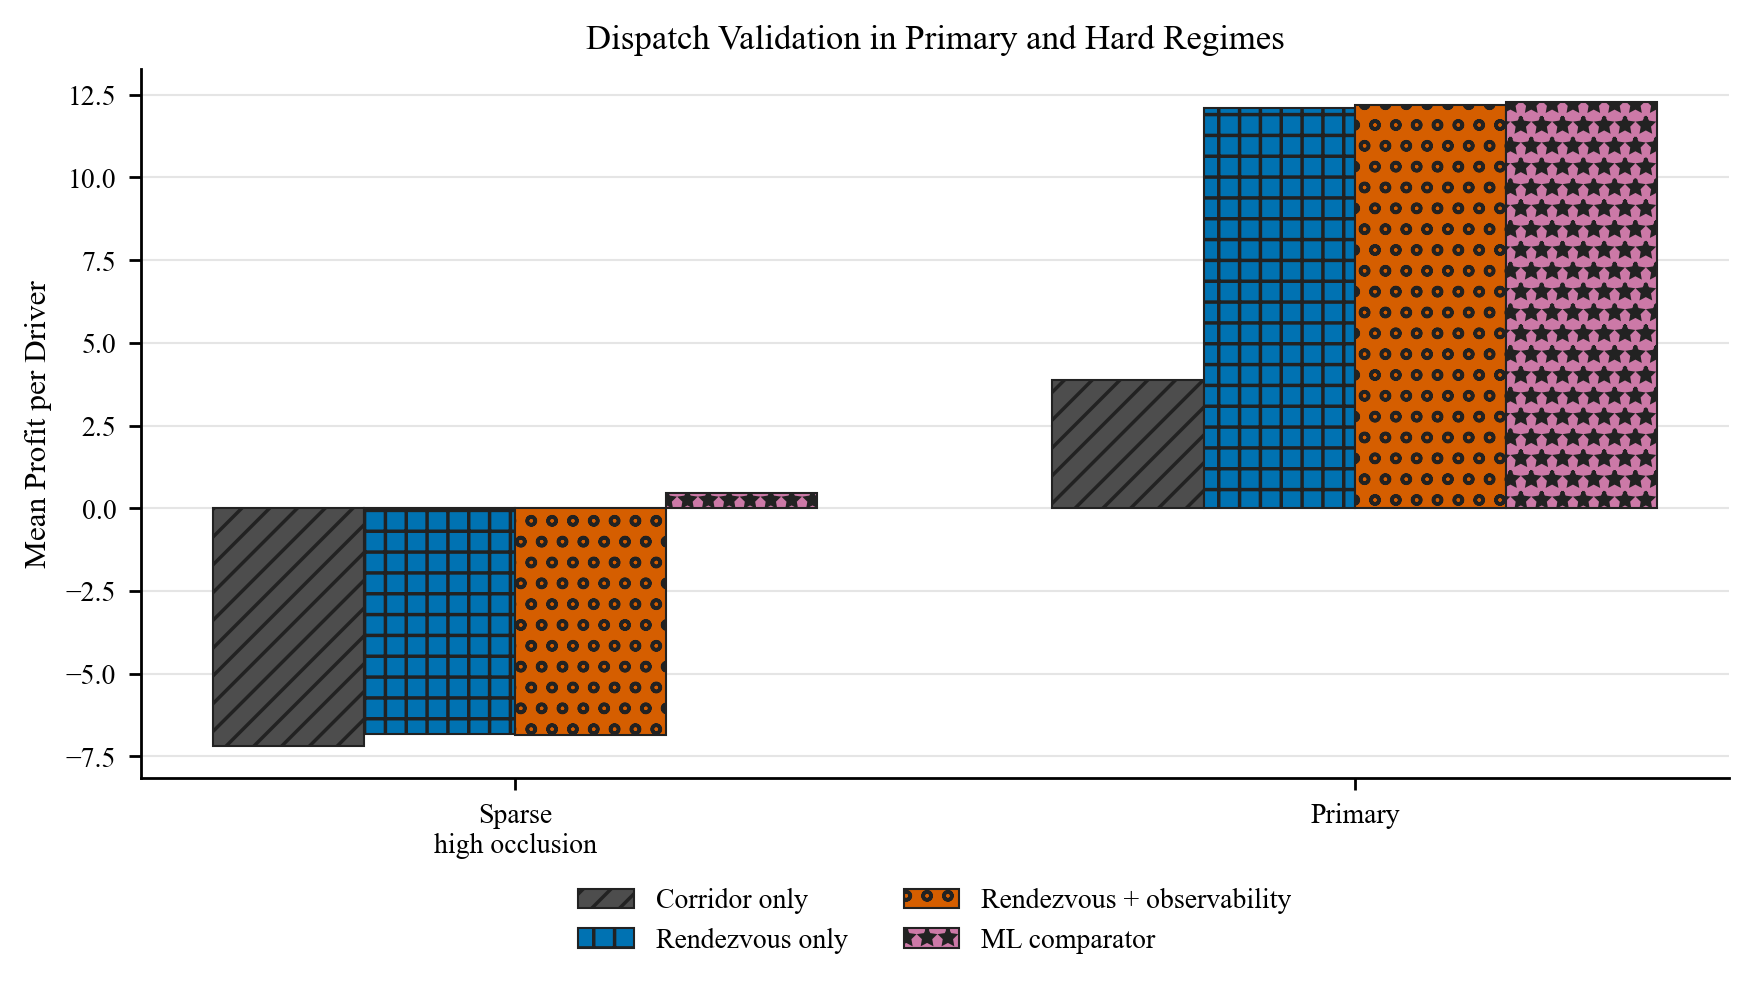
\includegraphics[width=\columnwidth]{figures/rendezvous_fig4_dispatch.png}
\caption{Dispatch validation in the primary and sparse high-occlusion regimes. The route-aware ordering survives under shared rider competition.}
\label{fig:dispatch}
\end{figure}

\subsection{Robustness and Ablation}
The robustness pass sharpens the paper's main claim. Figure~\ref{fig:timeslice} compares all-day, morning-peak, and evening-peak slices in sparse high occlusion. Morning peak is clearly harsher: mean actual profit falls to -4.57 for \texttt{corridor\_only}, -1.96 for \texttt{rendezvous\_only}, and -1.66 for \texttt{rendezvous\_observable}. Evening peak is easier, and the two rendezvous-aware deterministic policies are nearly tied at 7.62 and 7.60. This is exactly the regime-dependent pattern the paper claims: observability helps more when the operating slice is harder.

The urban-context ablation in Figure~\ref{fig:contextablation} is the cleanest observability-specific evidence in the study. In the earlier easier hard-regime slice, turning urban context off lowered \texttt{rendezvous\_only} from 5.52 to 5.05 and \texttt{rendezvous\_observable} from 5.72 to 5.19. The conclusion is not that every hand-crafted component weight is optimal, but that the urban-context layer materially improves hard-regime opportunity valuation when the route-choice problem is close.

Green transfer adds a second-domain check. Figure~\ref{fig:green} shows that the route-ordering hierarchy largely transfers without recalibration of the observability weights. In Green primary, \texttt{corridor\_only} stays near break-even at -0.00 while \texttt{rendezvous\_only} and \texttt{rendezvous\_observable} reach 4.32 and 4.31. In Green sparse high occlusion, \texttt{corridor\_only} drops to -6.56 while the rendezvous-aware policies improve to -6.04 and -6.10. Observability does not dominate on Green, but corridor-only valuation remains decisively weakest and the feasible-rendezvous framing transfers cleanly.

Figure~\ref{fig:sensitivity} then shows the boundary cases. In very sparse low occlusion, \texttt{walk\_aware\_rendezvous} and the ML comparator slightly edge the deterministic observability policy. In very sparse extreme occlusion, \texttt{rendezvous\_only} slightly edges \texttt{rendezvous\_observable}. These are not failures; they are exactly why the paper should be framed as a hard-regime systems contribution rather than as a universal dominance claim.
\par
The curated case-study layer in Figure~\ref{fig:casestudies} provides a local-geometry sanity check. Across eight selected route pairs, the fixed rubric agrees with the observability-aware preference in all eight cases, with several ties and several clear wins for the higher-observability route. The important point is not that the rubric is a new learned model; it is that local overlays built from building footprints, sidewalks, route anchors, and selected anchors are visually consistent with the route ranking the quantitative model prefers.
\begin{figure}[t]
\centering
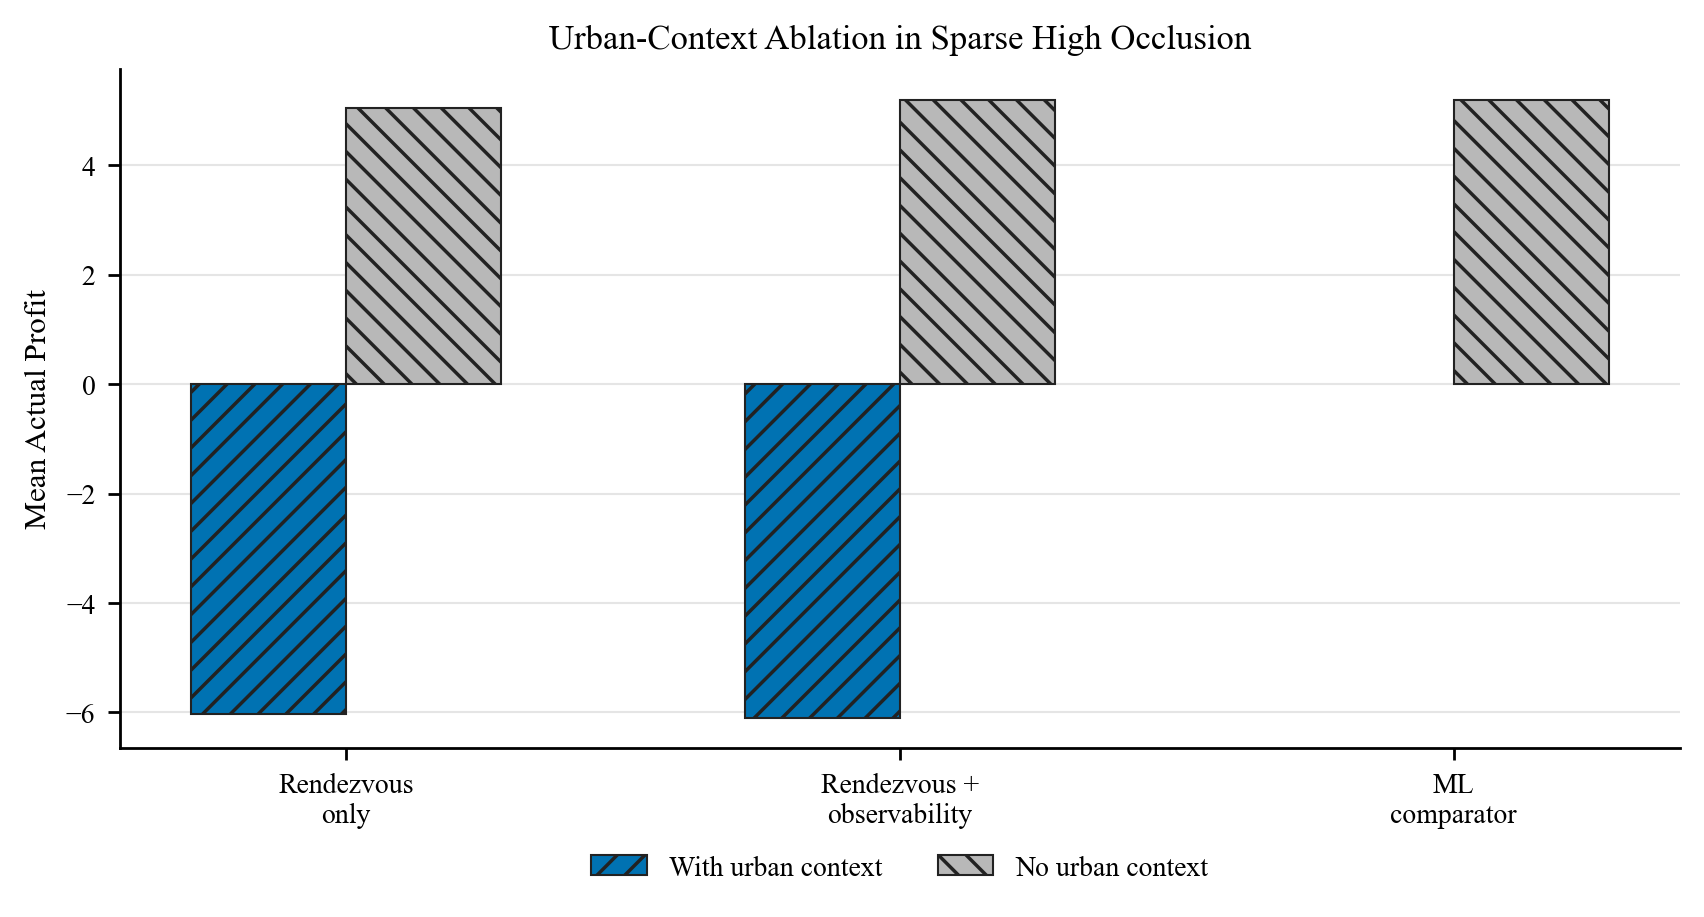
\includegraphics[width=\columnwidth]{figures/rendezvous_fig8_context_ablation.png}
\caption{Urban-context ablation in sparse high occlusion. Context helps the rendezvous-aware policies in the headline hard regime.}
\label{fig:contextablation}
\end{figure}

\begin{figure}[t]
\centering
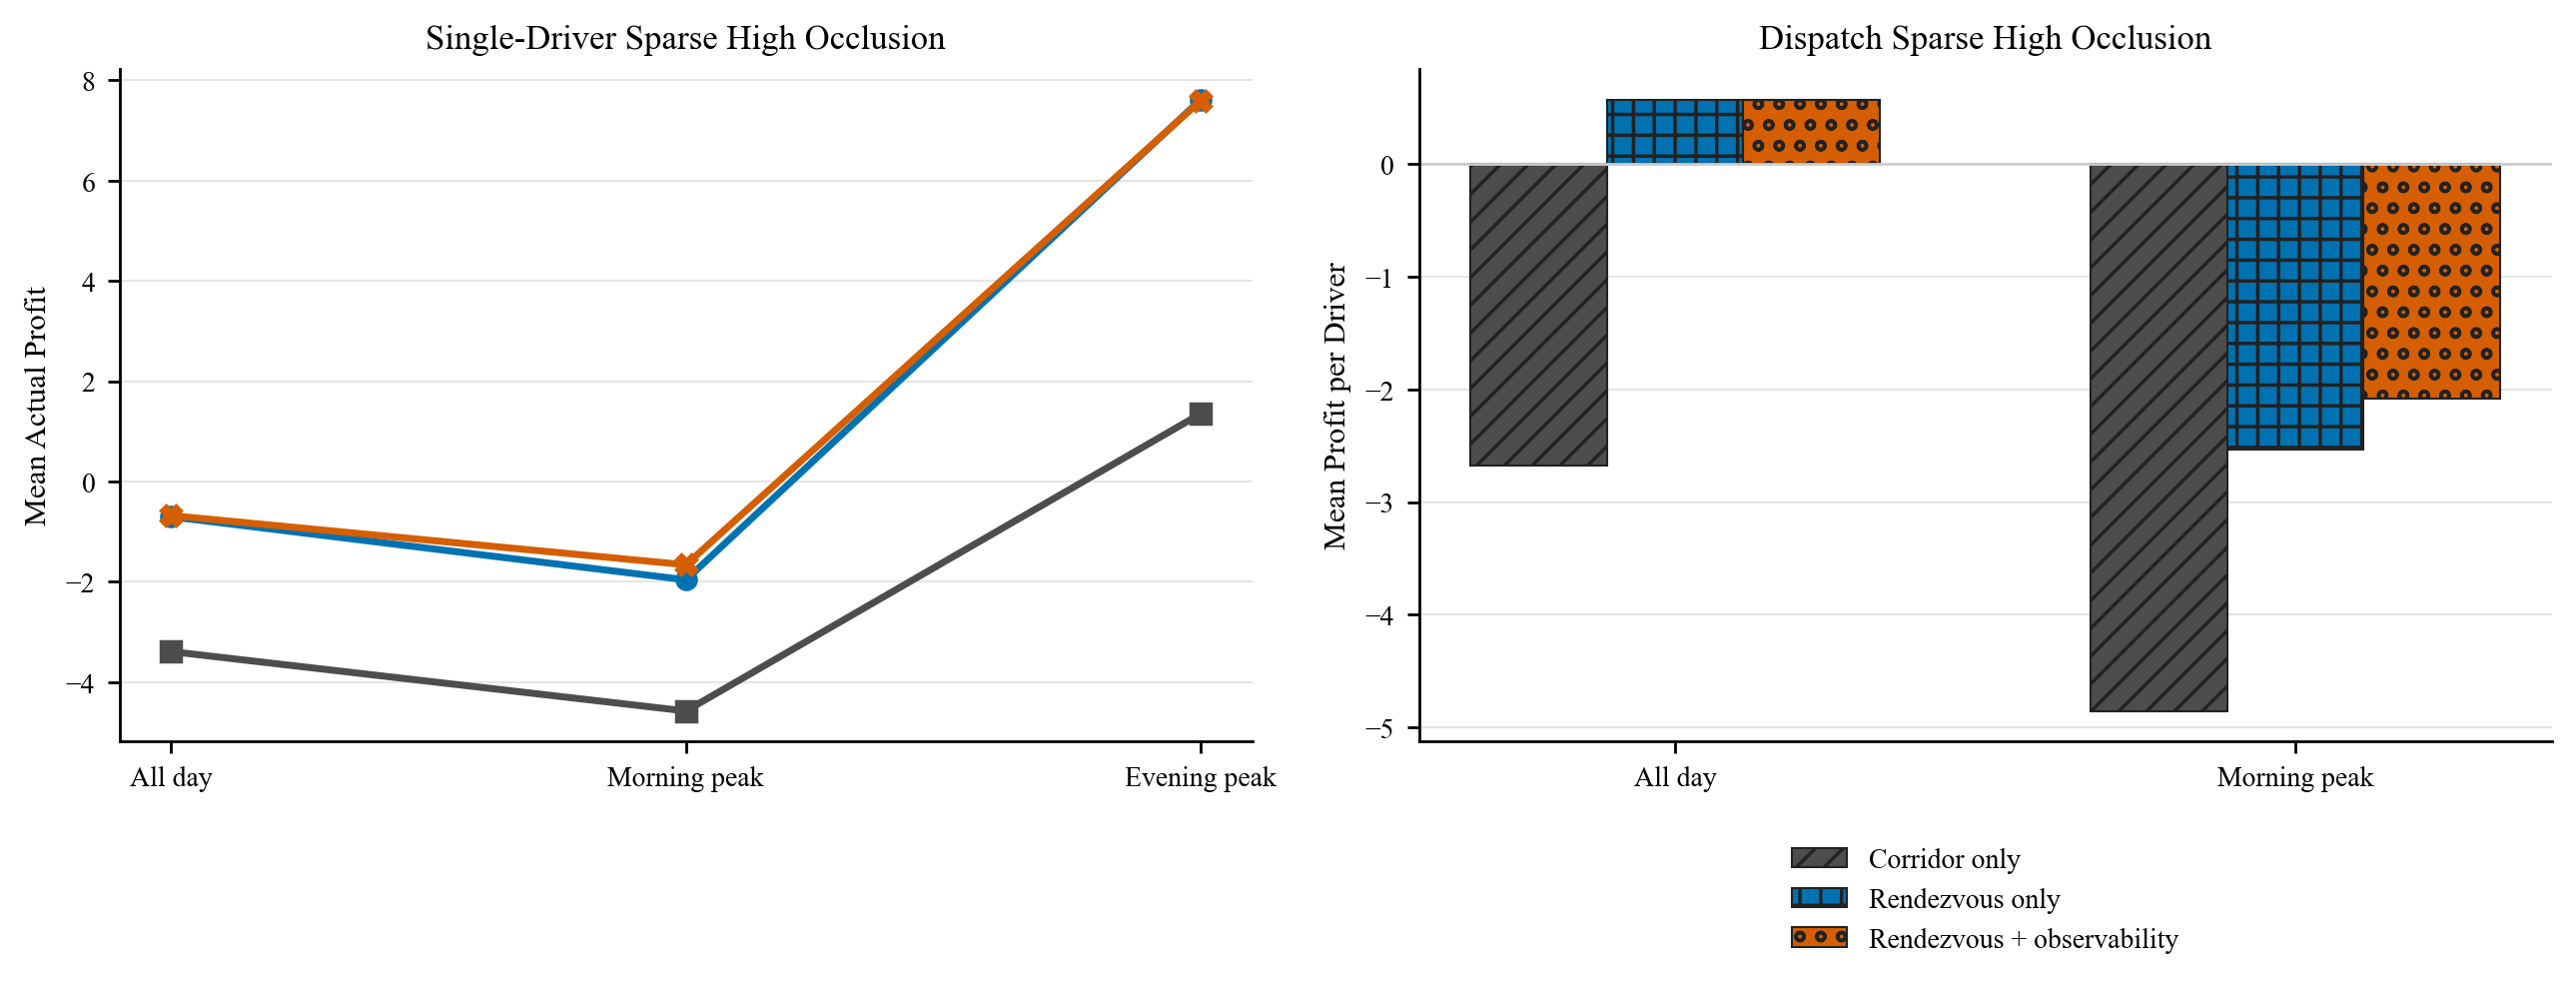
\includegraphics[width=\columnwidth]{figures/rendezvous_fig9_time_slice_robustness.png}
\caption{Time-slice robustness in sparse high occlusion. Morning peak is harder than all day, and the observability-aware deterministic policy is strongest in that slice.}
\label{fig:timeslice}
\end{figure}

\begin{figure}[t]
\centering
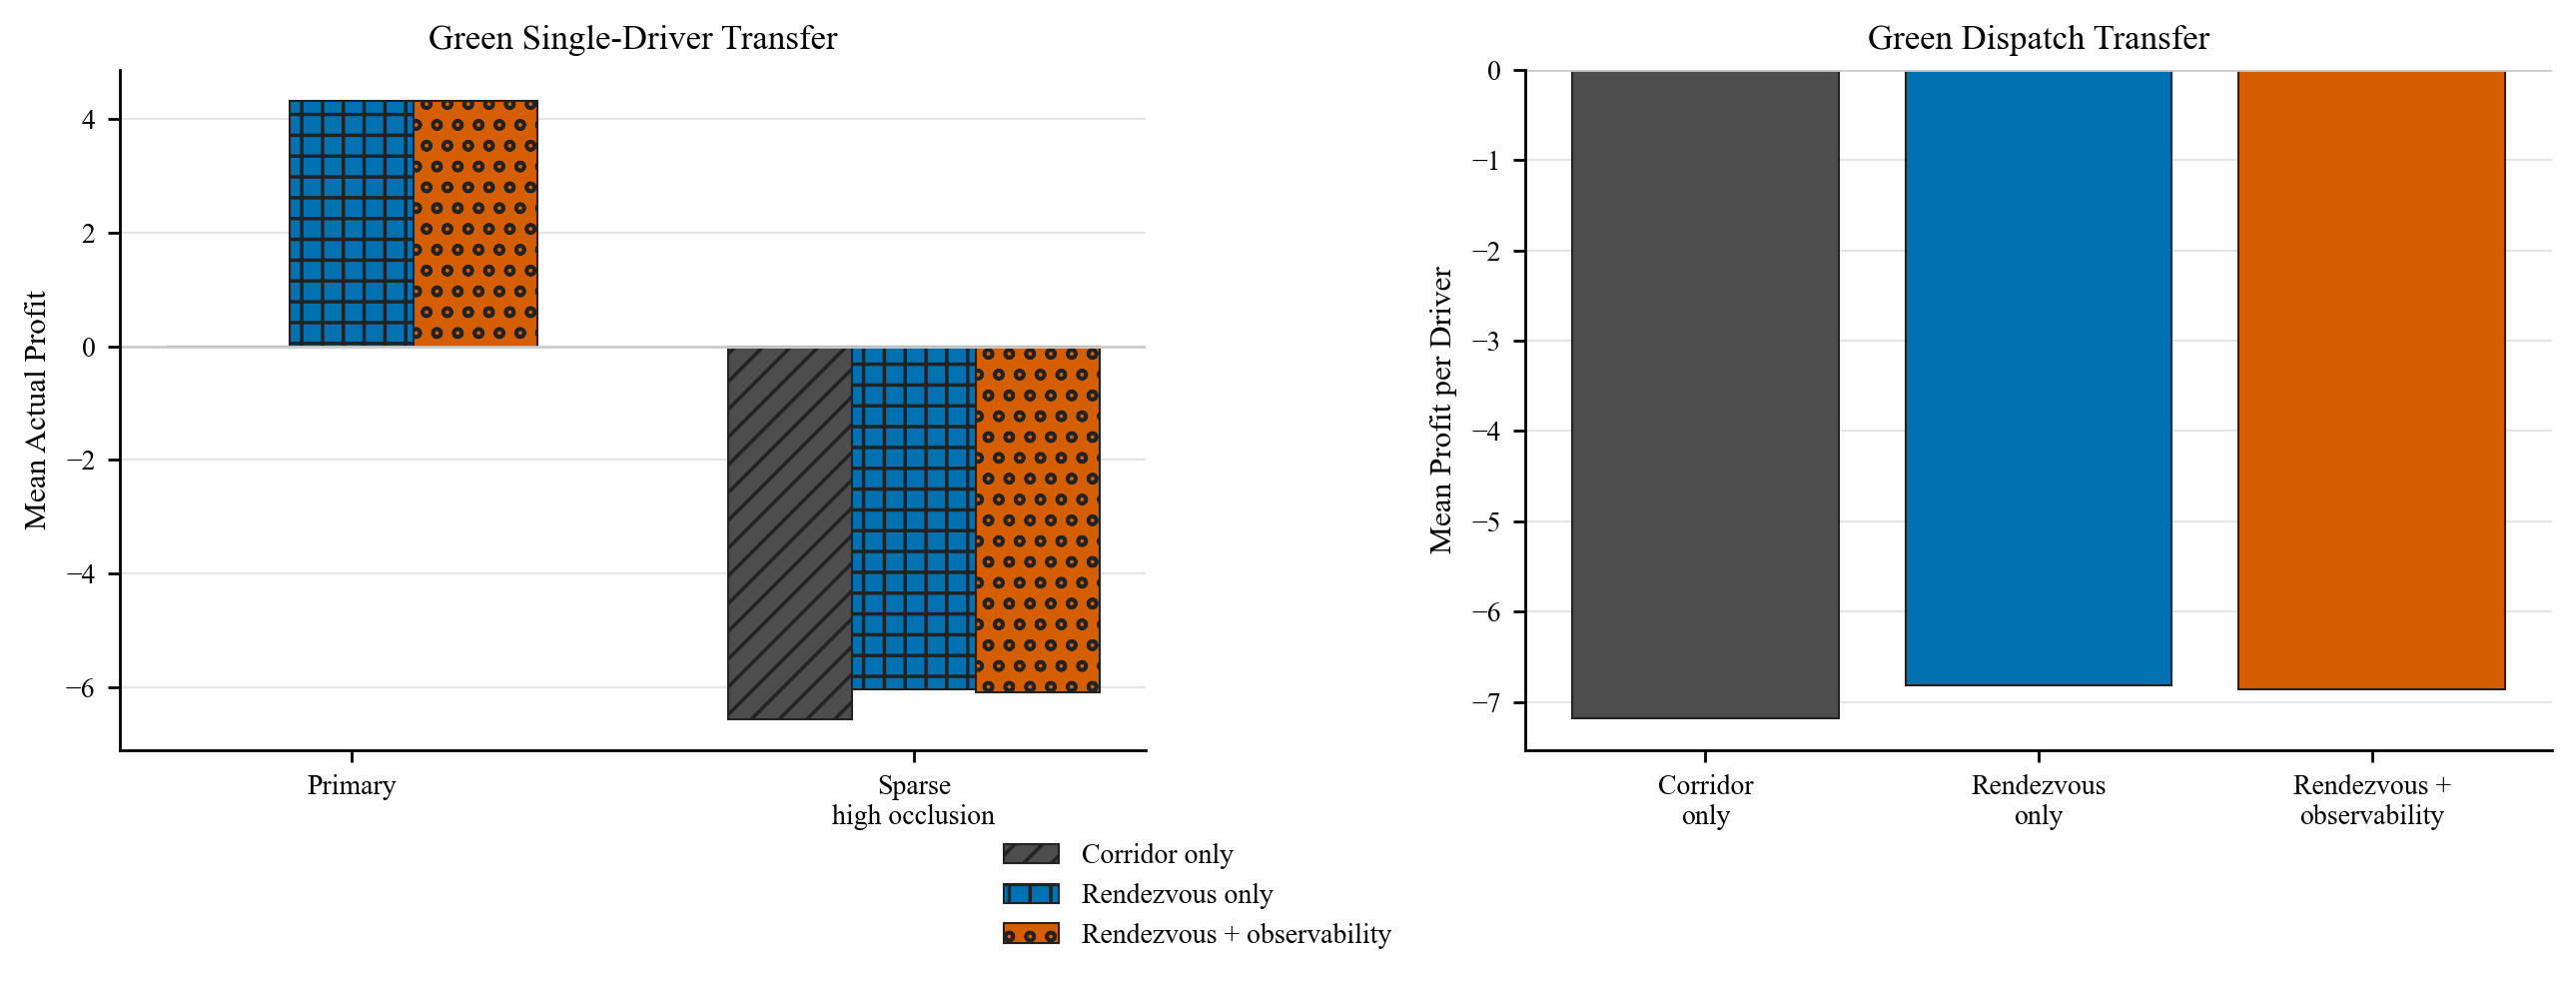
\includegraphics[width=\columnwidth]{figures/rendezvous_fig8_green_robustness.png}
\caption{Green-domain transfer. Corridor-only valuation remains weakest, while the feasible-rendezvous framing transfers more cleanly than a universal observability-win story.}
\label{fig:green}
\end{figure}

\begin{figure}[t]
\centering
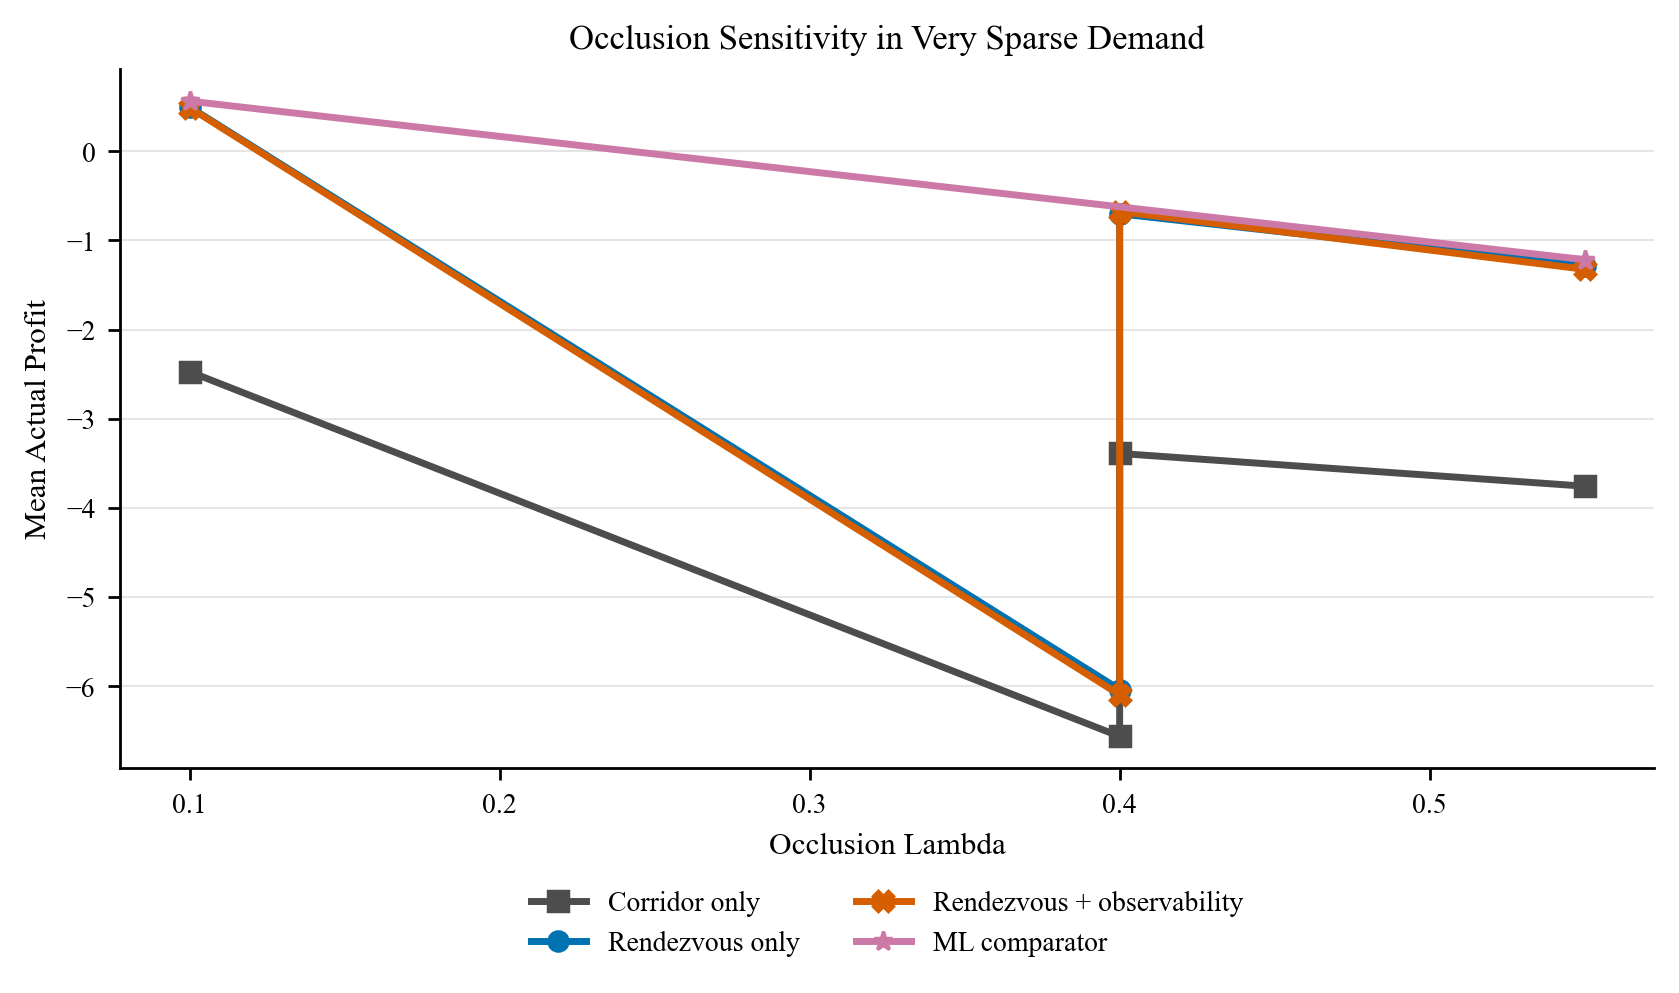
\includegraphics[width=\columnwidth]{figures/rendezvous_fig6_sensitivity.png}
\caption{Sensitivity in the very-sparse regimes. Observability-aware valuation is useful, but not uniformly dominant in every boundary case.}
\label{fig:sensitivity}
\end{figure}

\begin{figure}[t]
\centering
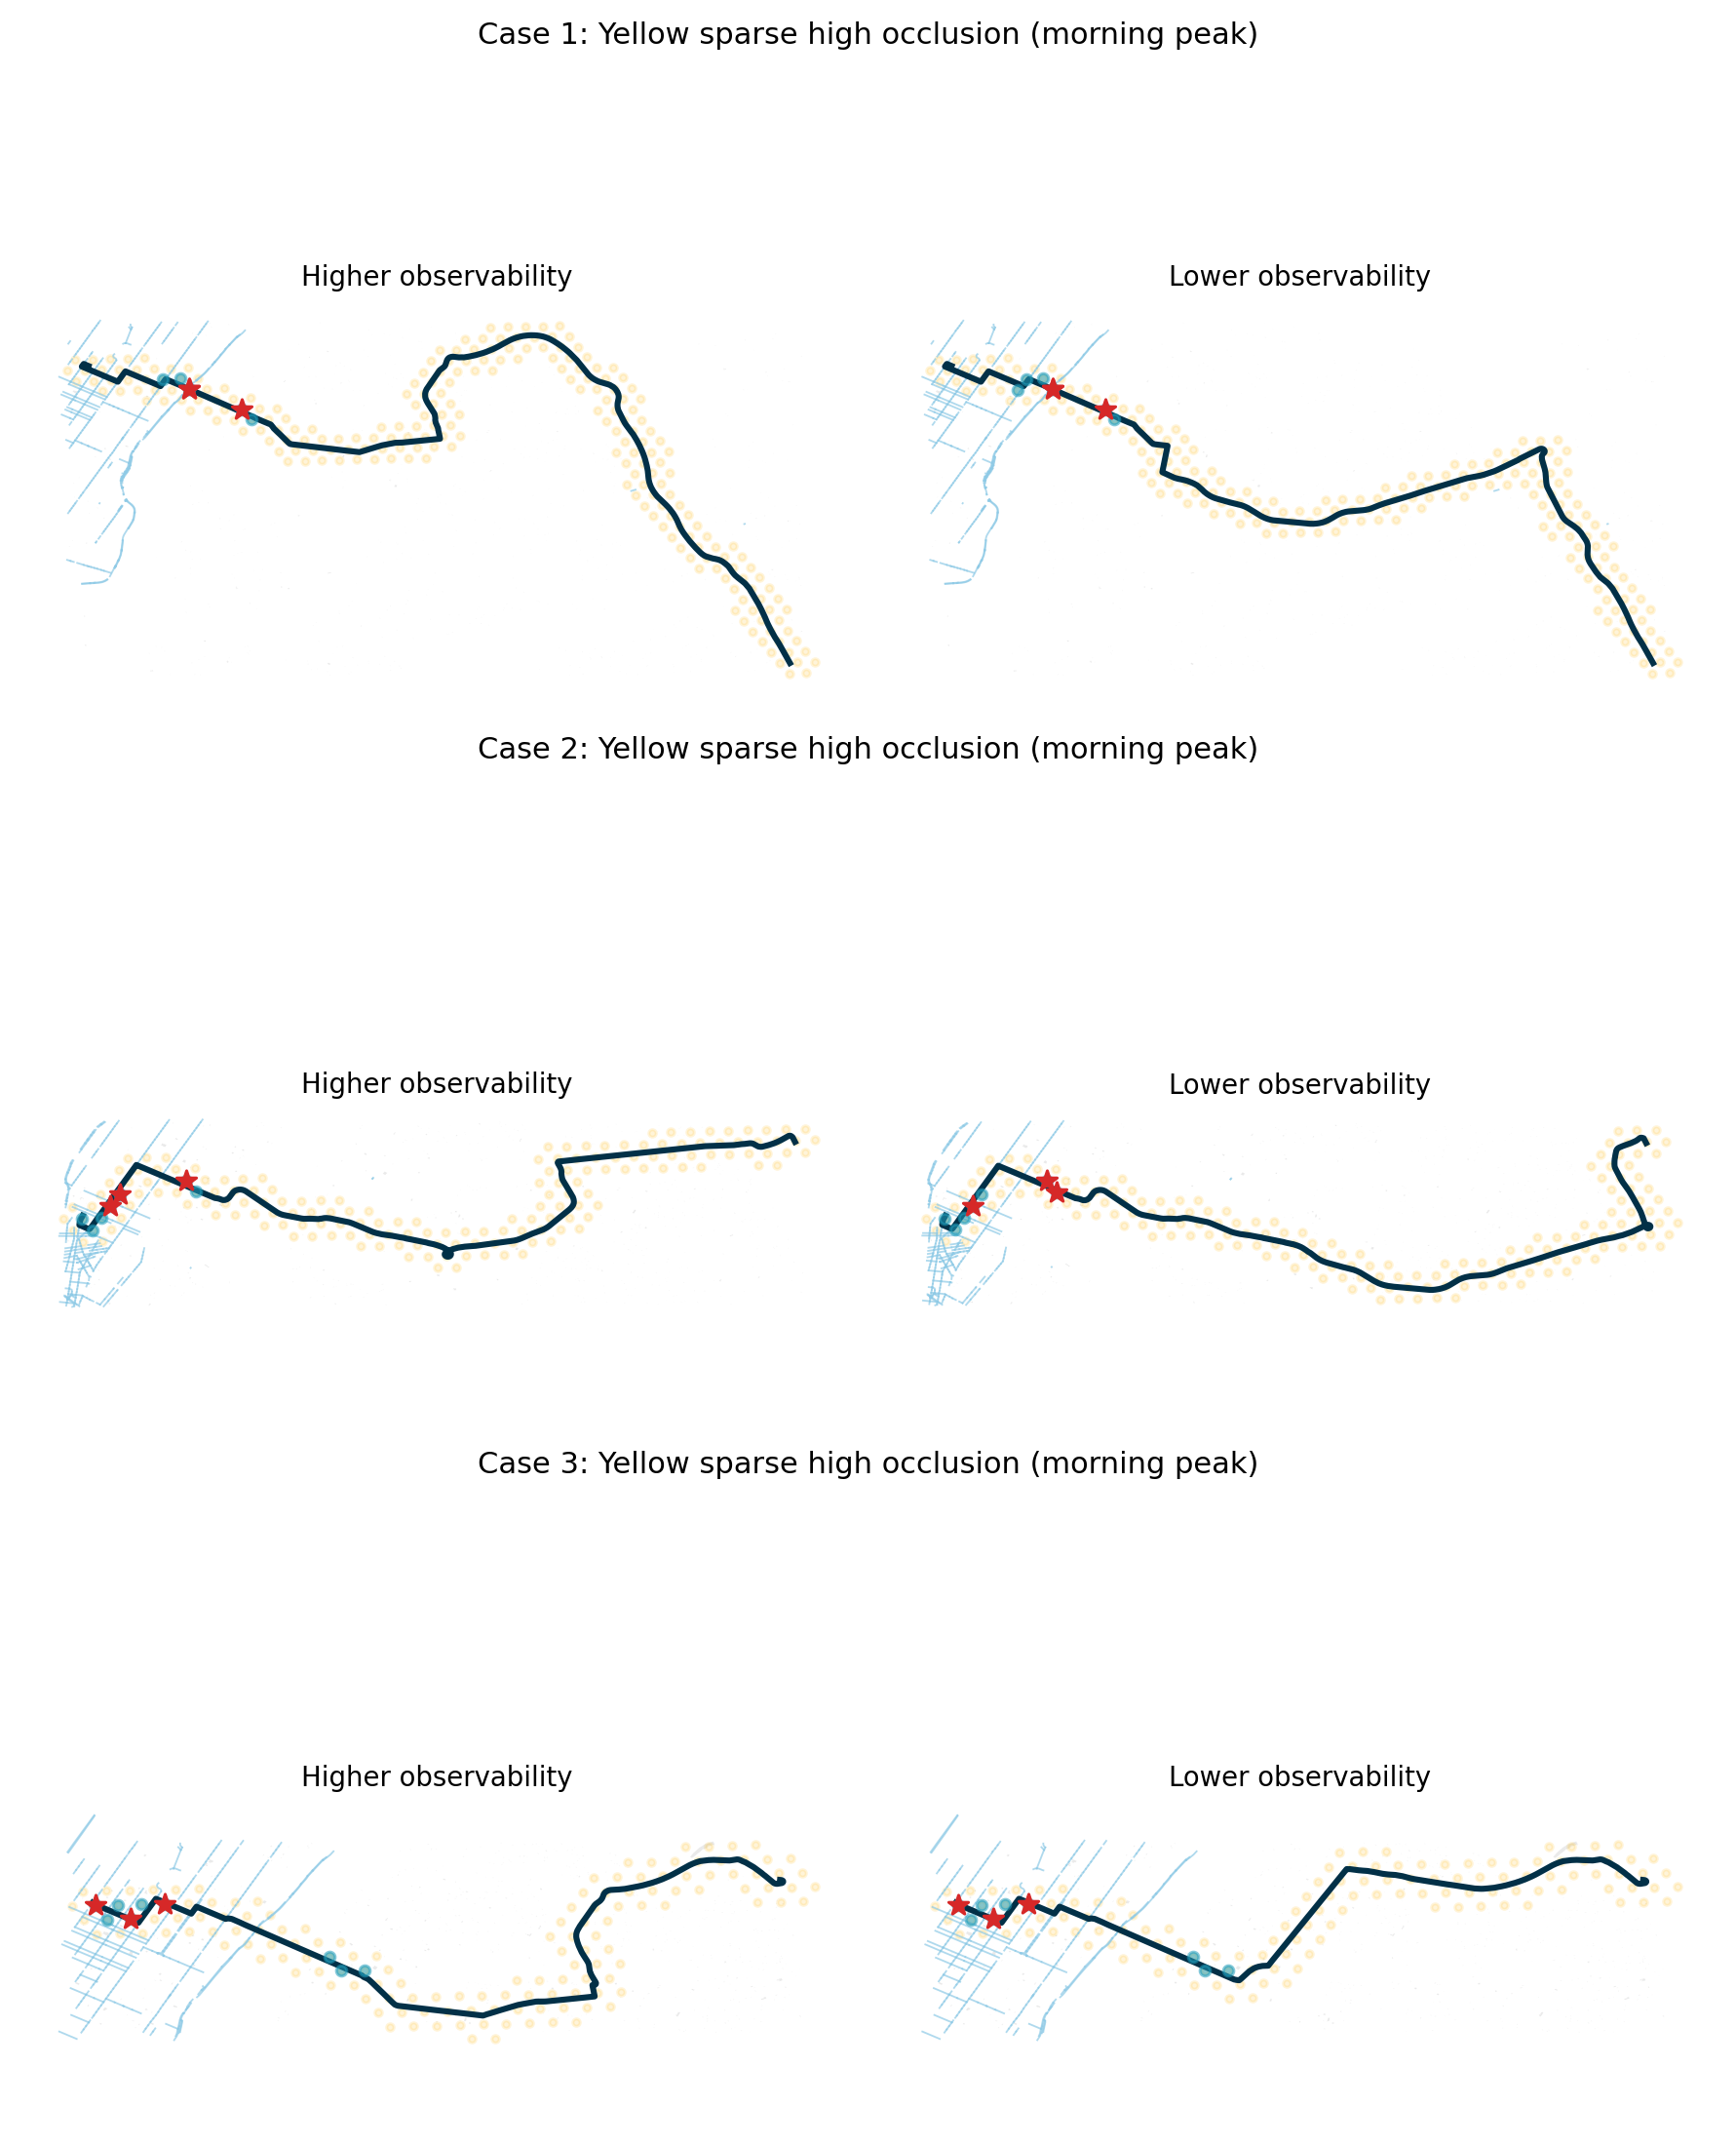
\includegraphics[width=\columnwidth]{figures/rendezvous_fig9_case_studies.png}
\caption{Curated local-geometry case studies. The highlighted route pairs have similar opportunity volume but visibly different anchor quality, sidewalk context, and local openness.}
\label{fig:casestudies}
\end{figure}

\subsection{ML Comparator}
The ML comparator remains secondary. Figure~\ref{fig:ml} shows that it is often competitive and sometimes strongest overall, but the supporting predictive diagnostics are modest: validation observed ROC AUC is 0.65 and test observed ROC AUC is 0.56. That is enough to justify keeping the comparator in the paper, but not enough to make it the paper's central method. The main scientific result remains the deterministic route-valuation comparison.

\begin{figure}[t]
\centering
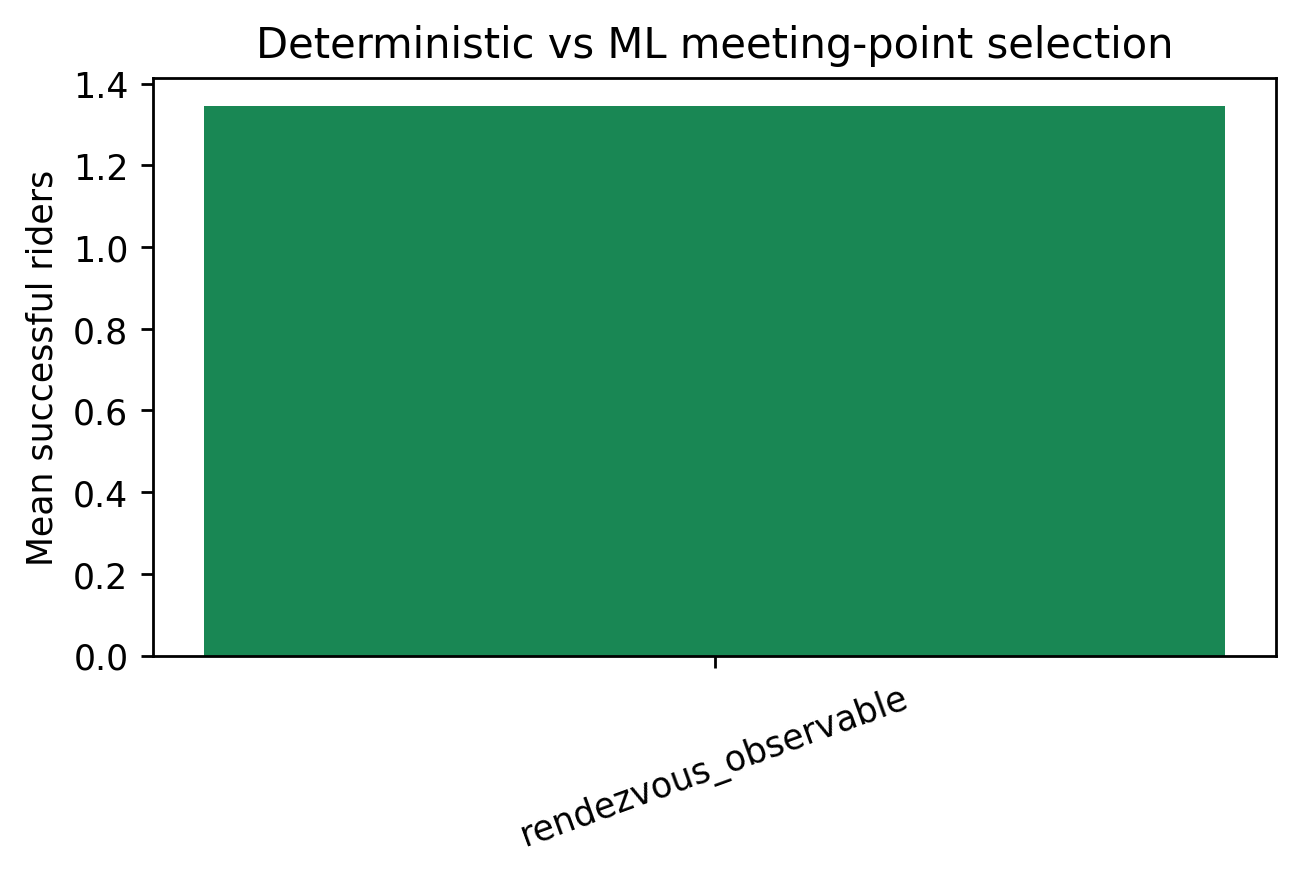
\includegraphics[width=\columnwidth]{figures/rendezvous_fig5_ml_comparator.png}
\caption{Deterministic observability-aware valuation versus the ML meeting-point comparator. The comparator is competitive, but the paper should remain centered on the deterministic route-valuation story.}
\label{fig:ml}
\end{figure}

\begin{table}[t]
\caption{Headline deterministic policy comparison on the default calibrated slice.}
\label{tab:headline}
\centering
\footnotesize
\begin{tabularx}{\columnwidth}{L{0.34\columnwidth}XXX}
\toprule
Setting & Corridor only & Rendezvous only & Rendezvous + obs. \\
\midrule
Single-driver primary & 6.76 & 17.60 & 17.57 \\
Single-driver sparse high occlusion & -3.39 & -0.70 & -0.68 \\
Dispatch primary & 3.87 & 12.10 & 12.19 \\
Dispatch sparse high occlusion & -2.67 & 0.57 & 0.57 \\
\bottomrule
\end{tabularx}
\end{table}

\section{Discussion}
The empirical pattern supports three substantive conclusions.

First, the paper's primitive shift is justified. Near-route riders are not the right unit for route evaluation when operational reality depends on shared meeting opportunities. The large corridor-only nominal-versus-realized gap is the clearest evidence for that claim.

Second, rendezvous feasibility is the major performance jump. This is important for positioning. The strongest deterministic gain in the study does not come from a complex observability model alone; it comes first from replacing corridor exposure with feasible common meeting opportunities.

Third, observability is useful in a structured, regime-dependent way. It is most helpful in sparse, high-occlusion settings and in the harsher morning-peak slice of that regime. That is a publishable and operationally meaningful result even though observability-aware valuation is not uniformly best in every boundary case.

This also clarifies the reviewer-risk story. The observability layer is still proxy-based, so the paper should not claim to solve perception. Instead, the stronger case is that the proxy is decision-relevant: it changes matched route ordering in Yellow hard-regime pairs, the feasible-rendezvous hierarchy transfers to Green without retuning, and the local geometry overlays are directionally consistent with the observability-aware ranking. For an ITS/systems paper, that combination is enough to support a route-choice claim without pretending to deliver a full sensor-physics model.

These points also clarify how this paper should be positioned relative to the earlier corridor paper. The earlier route-aware work showed that route choice matters because different corridors expose different rider pools. The present paper goes one level deeper: routes matter because they expose different \emph{meeting opportunities}, and those opportunities differ not only in accessibility but also in reliability under urban morphology. The scientific center of gravity is therefore distinct even though the implementation reuses infrastructure.

\section{Limitations}
The study remains bounded in several ways.
\begin{enumerate}
\item The observability layer is a structured proxy rather than a full physical sensing model.
\item The calibration improves discipline more than performance; it should not be oversold as a strong learning result.
\item The ML comparator is secondary and supported by only modest held-out observed-success discrimination.
\item The Green robustness layer improves transfer coverage, but the study is still NYC-only rather than cross-city.
\item The dispatch validation is intentionally smaller than the single-driver study and is used as secondary evidence rather than as the sole basis for the paper's claims.
\end{enumerate}

These limitations narrow the paper's scope, but they also sharpen it. The contribution is not a claim to solve dispatch, perception, or flexible pickup design in general. It is a more focused claim about how route value should be measured in ride-pooling when meeting opportunities and urban observability are made explicit.

\section{Conclusion}
This paper studies route choice in urban ride-pooling through route-induced rendezvous opportunities under occlusion. The main conclusion is that corridor exposure alone is not an adequate primitive for route evaluation. Routes should instead be valued by the feasible common meeting opportunities they create, and in harder urban regimes those opportunities should be further weighted by observability and pickup reliability.

The evaluation supports that conclusion in two complementary ways. In the controlled single-driver study, corridor-only valuation is decisively weakest and rendezvous-aware valuation is substantially stronger. In the repaired rolling-dispatch validation, the same qualitative ordering survives rider exclusivity and failed-attempt retirement. The observability-aware deterministic policy is strongest in the headline sparse high-occlusion regime and in the harder morning-peak slice, while boundary cases show that this advantage is regime-dependent rather than universal.

The broader implication is methodological as much as operational: route-aware ride-pooling studies should not collapse route value to proximity alone. They should treat feasible and observable rendezvous opportunities as the decision-relevant unit. That shift is the main contribution of the paper.

\bibliographystyle{IEEEtran}
\bibliography{references}
\end{document}
